\documentclass[12pt,a4paper]{article}

\usepackage[a4paper,margin=1in]{geometry}
\usepackage{graphicx}
\graphicspath{{../output_plots/}}
\usepackage{booktabs}
\usepackage{amsmath,amssymb}
\usepackage{float}
\usepackage{hyperref}
\usepackage{xcolor}
\usepackage{listings}
\usepackage{enumitem}
\usepackage{fancyhdr}
\usepackage{longtable}

\hypersetup{colorlinks=true,linkcolor=blue,urlcolor=blue}

\pagestyle{fancy}
\fancyhf{}
\lhead{ICS1512}
\rhead{Machine Learning Algorithms Laboratory}
\cfoot{\thepage}

\lstset{
language=Python,
basicstyle=\ttfamily\small,
numbers=left,
frame=single,
breaklines=true,
showstringspaces=false
}

\begin{document}

\begin{tabular}{|p{4cm}|p{11cm}|}
\hline
Experiment No. & 5 \\ \hline
Experiment Title & Decision Tree and Random Forest: A Comparative Classification Study\footnotemark \\ \hline
Student Name & Danusu K \\ \hline
Register Number & 3122247001013 \\ \hline
Faculty & Dr. Poreddy Ajay Kumar Reddy \\ \hline
Submission Date & \today \\ \hline
\end{tabular}
\footnotetext{\textbf{GitHub Repository: }\url{https://github.com/Danush-k/Machine-Learning}}

\section{Objective}
\begin{itemize}
\item To implement a \textbf{Decision Tree} classifier using tree-based recursive binary splitting.
\item To extend the single Decision Tree into a \textbf{Random Forest} ensemble model via bootstrap aggregation (bagging) and random feature subspace selection.
\item To systematically study the impact of hyperparameters (maximum depth, impurity criteria, min samples split, min samples leaf, and number of estimators) on model overfitting and generalization.
\item To select optimal hyperparameters using \textbf{5-Fold Stratified Cross-Validation}.
\item To evaluate and compare single-tree and ensemble-tree models using standard classification metrics (Accuracy, Precision, Recall, F1-score, Confusion Matrix, ROC-AUC, and Gini Feature Importance).
\end{itemize}

\section{Problem Statement}
Breast cancer is among the most prevalent malignancies worldwide, and automated, computer-aided diagnostic (CAD) systems provide vital secondary opinions for clinical practitioners. The objective of this study is to formulate and benchmark supervised classification models to categorize digitized Fine Needle Aspirate (FNA) cell nuclei images into either \textbf{Benign ($y=0$)} or \textbf{Malignant ($y=1$)}. Using the 30 continuous real-valued geometric and morphometric attributes from the Wisconsin Diagnostic Breast Cancer (WDBC) dataset, we contrast a single interpretable Decision Tree with a robust, variance-reduced Random Forest ensemble. The models must maximize diagnostic sensitivity (Recall) while maintaining high overall precision and low generalization variance under 5-Fold Cross-Validation.

\section{Dataset Description}
\begin{longtable}{|p{6cm}|p{8cm}|}
\hline
Dataset Name & Wisconsin Diagnostic Breast Cancer (WDBC) \\ \hline
Dataset Source & UCI Machine Learning Repository \\ \hline
Total Number of Samples & 569 patient instances \\ \hline
Number of Attributes & 32 (ID, Diagnosis target, 30 continuous numerical features) \\ \hline
Target Classes & 2 (Binary: $B = \text{Benign} \, (0)$, $M = \text{Malignant} \, (1)$) \\ \hline
Class Distribution & 357 Benign (62.74\%), 212 Malignant (37.26\%) \\ \hline
Missing Values & 0 (Complete dataset) \\ \hline
Train-Test Split & 80\% Training (455 samples), 20\% Testing (114 samples) \\ \hline
\end{longtable}

The 30 continuous numerical features are derived from 10 fundamental characteristics computed for each cell nucleus:
\begin{enumerate}[label=(\alph*)]
\item Radius (mean of distances from center to perimeter points)
\item Texture (standard deviation of gray-scale values)
\item Perimeter
\item Area
\item Smoothness (local variation in radius lengths)
\item Compactness ($\frac{\text{perimeter}^2}{\text{area}} - 1.0$)
\item Concavity (severity of concave portions of the contour)
\item Concave Points (number of concave portions of the contour)
\item Symmetry
\item Fractal Dimension (``coastline approximation'' $- 1$)
\end{enumerate}
For each image, the \textbf{Mean}, \textbf{Standard Error (SE)}, and \textbf{Worst (largest)} values of these 10 metrics were computed, yielding $3 \times 10 = 30$ input features.

\section{Exploratory Data Analysis}
Exploratory data analysis was conducted to examine the distribution of diagnostic target labels and quantify the linear associations between morphometric nuclear attributes and tumor malignancy.

\begin{figure}[H]
\centering

\includegraphics[width=0.85\linewidth]{01_class_distribution.png}
\caption{Class Distribution of WDBC Dataset (Benign vs Malignant)}
\end{figure}

\textbf{Inference:}
The dataset consists of 569 biopsy samples, comprising 357 Benign tumors (62.74\%) and 212 Malignant tumors (37.26\%). The class ratio is approximately $1.68 : 1$, indicating a mild class imbalance. Stratified sampling is employed during train-test splitting and $K$-fold partitioning to preserve these exact class proportions across all cross-validation folds, preventing split-induced sampling bias.

\begin{figure}[H]
\centering

\includegraphics[width=0.85\linewidth]{02_feature_correlation.png}
\caption{Top 15 Features Ranked by Absolute Pearson Correlation with Malignancy}
\end{figure}

\textbf{Inference:}
The correlation analysis highlights that nuclear contour attributes, specifically \texttt{concave\_points\_worst} ($|r| = 0.794$), \texttt{perimeter\_worst} ($|r| = 0.783$), \texttt{concave\_points\_mean} ($|r| = 0.777$), and \texttt{radius\_worst} ($|r| = 0.776$), exhibit the strongest positive linear correlations with breast cancer malignancy. Malignant nuclei consistently present enlarged diameters, irregular contours, and extensive concavities. These highly correlated attributes serve as primary split candidates near the root nodes in decision tree induction.

\section{Data Preprocessing}
\begin{itemize}
\item \textbf{Missing Value Analysis:} Checked dataset integrity across all 569 rows and 30 numerical features; confirmed zero missing, NaN, or null values.
\item \textbf{Target Encoding:} Encoded categorical clinical diagnosis labels into binary integer format: $\text{Benign (B)} \rightarrow 0$ and $\text{Malignant (M)} \rightarrow 1$.
\item \textbf{Scale Invariance:} Tree-based algorithms (Decision Trees and Random Forests) make orthogonal axis-parallel partition cuts based on monotonic ranking of individual feature values; hence, feature scaling (Standardization or Min-Max normalization) does not alter tree topology or split points, preserving raw feature interpretability.
\item \textbf{Stratified Train-Test Split:} Partitioned the 569 samples into an 80\% training set (455 samples) and a 20\% held-out test set (114 samples) using stratified random sampling with fixed seed $\text{random\_state}=42$.
\end{itemize}

\section{Machine Learning Algorithm}

\subsection{Decision Tree Classifier}
A Decision Tree recursively partitions the input space $\mathbb{R}^p$ into hyper-rectangles by selecting at each internal node the feature $j$ and split threshold $t$ that maximize the reduction in impurity (Information Gain).
\begin{itemize}
\item \textbf{Gini Impurity:}
\begin{equation}
I_G(D) = 1 - \sum_{k=1}^K p_k^2
\end{equation}
where $p_k$ is the proportion of training instances belonging to class $k$ in node $D$.
\item \textbf{Entropy \& Information Gain:}
\begin{equation}
H(D) = -\sum_{k=1}^K p_k \log_2 (p_k)
\end{equation}
\begin{equation}
\Delta H(D, j, t) = H(D) - \frac{|D_L|}{|D|} H(D_L) - \frac{|D_R|}{|D|} H(D_R)
\end{equation}
where $D_L = \{(\mathbf{x}, y) \in D \mid x_j \le t\}$ and $D_R = \{(\mathbf{x}, y) \in D \mid x_j > t\}$.
\item \textbf{Overfitting Limitation:} Unconstrained, deep decision trees recursively split until every leaf is pure ($I_G=0$), capturing idiosyncratic noise and outliers in the training data, leading to high model variance and poor out-of-sample generalization. Pre-pruning via \texttt{max\_depth}, \texttt{min\_samples\_split}, and \texttt{min\_samples\_leaf} is required to control complexity.
\end{itemize}

\subsection{Random Forest Classifier}
Random Forest is an ensemble learning method that constructs a collection of $B$ de-correlated decision trees $\{T_1, T_2, \dots, T_B\}$ and aggregates their predictions.
\begin{itemize}
\item \textbf{Bootstrap Aggregation (Bagging):} Each individual tree $T_b$ is trained on a bootstrap sample $D_b$ of size $N$ drawn uniformly with replacement from the training dataset $D$. Approximately $63.2\%$ of unique instances are included in each bootstrap sample, leaving $36.8\%$ as Out-of-Bag (OOB) data.
\item \textbf{Random Feature Subspace Selection:} At each candidate node split, only a random subset of $m$ features ($m \approx \sqrt{p}$) is evaluated rather than all $p$ features. This prevents dominant features from dictating every tree's root, yielding substantially de-correlated trees.
\item \textbf{Ensemble Prediction via Majority Voting:}
\begin{equation}
\hat{y}(\mathbf{x}) = \text{mode} \left( \{ T_b(\mathbf{x}) \}_{b=1}^B \right), \quad \hat{P}(y=1|\mathbf{x}) = \frac{1}{B} \sum_{b=1}^B T_b(\mathbf{x})
\end{equation}
\item \textbf{Theoretical Variance Reduction:} If $B$ individual trees each have variance $\sigma^2$ with pairwise correlation $\rho$, the variance of the ensemble average is:
\begin{equation}
\text{Var}\left(\frac{1}{B}\sum_{b=1}^B T_b\right) = \rho \sigma^2 + \frac{1-\rho}{B}\sigma^2
\end{equation}
As $B \to \infty$, the second term approaches zero, bounding ensemble variance strictly to $\rho \sigma^2$. Random feature selection reduces $\rho$, yielding lower total variance without increasing individual tree bias.
\end{itemize}

\section{Experimental Setup}
\begin{table}[H]
\centering
\begin{tabular}{ll}
\toprule
\textbf{Parameter / Component} & \textbf{Specification} \\
\midrule
Python Version & 3.11.15 \\
Scikit-Learn Version & 1.8.0 \\
IDE Environment & Antigravity IDE / VS Code \\
Operating System & macOS (Darwin arm64) \\
Processor / Hardware & Apple Silicon M-Series CPU / 16GB RAM \\
Cross-Validation Strategy & 5-Fold Stratified Cross-Validation \\
Random State Seed & 42 \\
\bottomrule
\end{tabular}
\caption{Hardware and Software Experimental Configuration}
\end{table}

\section{Hyperparameter Selection}

\subsection{Decision Tree Cross-Fold Results}
A comprehensive grid search was executed over impurity criteria (\texttt{gini}, \texttt{entropy}, \texttt{log\_loss}), maximum depth ($d \in [2, 10]$ and None), minimum samples split ($[2, 20]$), and minimum samples leaf ($[1, 8]$) using 5-Fold Stratified CV.

\begin{table}[H]
\centering
\small
\begin{tabular}{llcccc}
\toprule
\textbf{Criterion} & \textbf{Max Depth} & \textbf{Min Split} & \textbf{Min Leaf} & \textbf{Avg CV Accuracy (\%)} & \textbf{Avg CV F1 Score} \\
\midrule
Entropy & 4 (Optimal) & 2 & 2 & \textbf{94.07} & \textbf{0.9174} \\
Entropy & 3 & 2 & 2 & 93.63 & 0.9135 \\
Entropy & 5 & 2 & 2 & 93.63 & 0.9113 \\
Entropy & 6 & 2 & 2 & 93.63 & 0.9113 \\
Entropy & 8 & 2 & 2 & 93.63 & 0.9113 \\
Entropy & None (Unpruned) & 2 & 2 & 93.63 & 0.9113 \\
Entropy & 2 & 2 & 8 & 92.75 & 0.9009 \\
\midrule
Gini & 4 & 2 & 2 & 93.63 & 0.9126 \\
Gini & 3 & 2 & 4 & 93.19 & 0.9079 \\
Gini & 5 & 2 & 2 & 92.75 & 0.9022 \\
Gini & 6 & 2 & 2 & 92.75 & 0.9022 \\
Gini & None (Unpruned) & 2 & 2 & 92.75 & 0.9022 \\
Gini & 2 & 2 & 8 & 92.75 & 0.9009 \\
\midrule
Log Loss & 4 & 2 & 2 & \textbf{94.07} & \textbf{0.9174} \\
Log Loss & 3 & 2 & 2 & 93.63 & 0.9135 \\
Log Loss & 5 & 2 & 2 & 93.63 & 0.9113 \\
\bottomrule
\end{tabular}
\caption{Table 1: Decision Tree Hyperparameter Evaluation using 5-Fold Cross-Validation}
\end{table}

\subsection{Random Forest Cross-Fold Results}
Grid search optimization was conducted across the ensemble hyperparameter space including number of trees ($n\_estimators \in [25, 300]$), tree depth ($[3, 12]$ and None), maximum feature fraction ($[\sqrt{p}, \log_2 p, 0.5, \text{All}]$), and bootstrapping.

\begin{table}[H]
\centering
\small
\begin{tabular}{cccccc}
\toprule
\textbf{n\_estimators} & \textbf{Max Depth} & \textbf{Max Features} & \textbf{Bootstrap} & \textbf{Avg CV Accuracy (\%)} & \textbf{Avg CV F1 Score} \\
\midrule
25 & 12 & 0.5 (Optimal) & True & \textbf{97.58} & \textbf{0.9675} \\
100 & 8 & 0.5 & True & 97.36 & 0.9644 \\
200 & 12 & 0.5 & True & 97.36 & 0.9644 \\
300 & None & 0.5 & True & 97.36 & 0.9644 \\
100 & 5 & $\sqrt{p}$ & True & 96.92 & 0.9579 \\
200 & 8 & $\sqrt{p}$ & True & 96.92 & 0.9579 \\
300 & None & $\sqrt{p}$ & True & 96.92 & 0.9579 \\
50 & 5 & $\log_2 p$ & True & 96.70 & 0.9546 \\
100 & None & $\log_2 p$ & True & 96.70 & 0.9546 \\
25 & 3 & $\sqrt{p}$ & True & 95.82 & 0.9419 \\
\bottomrule
\end{tabular}
\caption{Table 2: Random Forest Hyperparameter Evaluation using 5-Fold Cross-Validation}
\end{table}

\subsection{Selected Optimal Hyperparameters}
\begin{table}[H]
\centering
\begin{tabular}{lll}
\toprule
\textbf{Model} & \textbf{Hyperparameter} & \textbf{Optimal Value} \\
\midrule
Decision Tree & Criterion & \texttt{'entropy'} (Information Gain) \\
Decision Tree & Max Depth & 4 \\
Decision Tree & Min Samples Split & 2 \\
Decision Tree & Min Samples Leaf & 2 \\
\midrule
Random Forest & Number of Estimators ($B$) & 25 (Stable from 25 to 300) \\
Random Forest & Max Depth & 12 \\
Random Forest & Max Features & 0.5 (15 features per split) \\
Random Forest & Bootstrap & True \\
\bottomrule
\end{tabular}
\caption{Optimal Hyperparameter Configurations Selected via 5-Fold CV}
\end{table}

\section{5-Fold Cross-Validation Performance Comparison}
The performance of the optimal single Decision Tree and Random Forest models across each of the 5 cross-validation folds is documented below.

\begin{table}[H]
\centering
\begin{tabular}{lccccccc}
\toprule
\textbf{Model} & \textbf{Fold 1} & \textbf{Fold 2} & \textbf{Fold 3} & \textbf{Fold 4} & \textbf{Fold 5} & \textbf{Average (\%)} & \textbf{Std Dev (\%)} \\
\midrule
Decision Tree & 93.41 & 95.60 & 90.11 & 95.60 & 95.60 & 94.07 & $\pm 2.15$ \\
Random Forest & 96.70 & 100.00 & 97.80 & 94.51 & 98.90 & \textbf{97.58} & $\mathbf{\pm 1.89}$ \\
\bottomrule
\end{tabular}
\caption{Table 3: 5-Fold Cross-Validation Accuracy Comparison}
\end{table}

\section{Final Test Set Results (Held-Out 20\% Partition)}
Models trained on the training partition with optimal hyperparameters were evaluated on the held-out test set ($N=114$).

\begin{table}[H]
\centering
\begin{tabular}{lcccccc}
\toprule
\textbf{Model} & \textbf{Accuracy} & \textbf{Precision} & \textbf{Recall} & \textbf{F1-score} & \textbf{ROC-AUC} & \textbf{Fit Time (s)} \\
\midrule
Decision Tree & 0.9298 & 1.0000 & 0.8095 & 0.8947 & 0.9563 & 0.0028 \\
Random Forest & \textbf{0.9737} & \textbf{1.0000} & \textbf{0.9286} & \textbf{0.9630} & \textbf{0.9902} & 0.0245 \\
\bottomrule
\end{tabular}
\caption{Comparative Test Set Performance Metrics}
\end{table}

\section{Result Visualization}

\begin{figure}[H]
\centering

\includegraphics[width=0.75\linewidth]{01_class_distribution.png}
\caption{Class Distribution of the WDBC Dataset}
\end{figure}
\textbf{Inference:}
The dataset contains 357 Benign cases (62.7\%) and 212 Malignant cases (37.3\%). Both classes possess substantial representation, enabling effective tree node splitting without severe majority-class starvation. Stratified splitting preserves this class proportion across both training and test partitions.

\begin{figure}[H]
\centering

\includegraphics[width=0.75\linewidth]{02_feature_correlation.png}
\caption{Top 15 Absolute Feature Correlations with Malignancy}
\end{figure}
\textbf{Inference:}
Attributes measuring cell boundary concavity and size (\texttt{concave\_points\_worst}, \texttt{perimeter\_worst}, \texttt{concave\_points\_mean}, \texttt{radius\_worst}) demonstrate strong correlation coefficients ($r > 0.77$). These features serve as the primary split variables in both models, providing high discriminative power to differentiate malignant from benign cytology.

\begin{figure}[H]
\centering
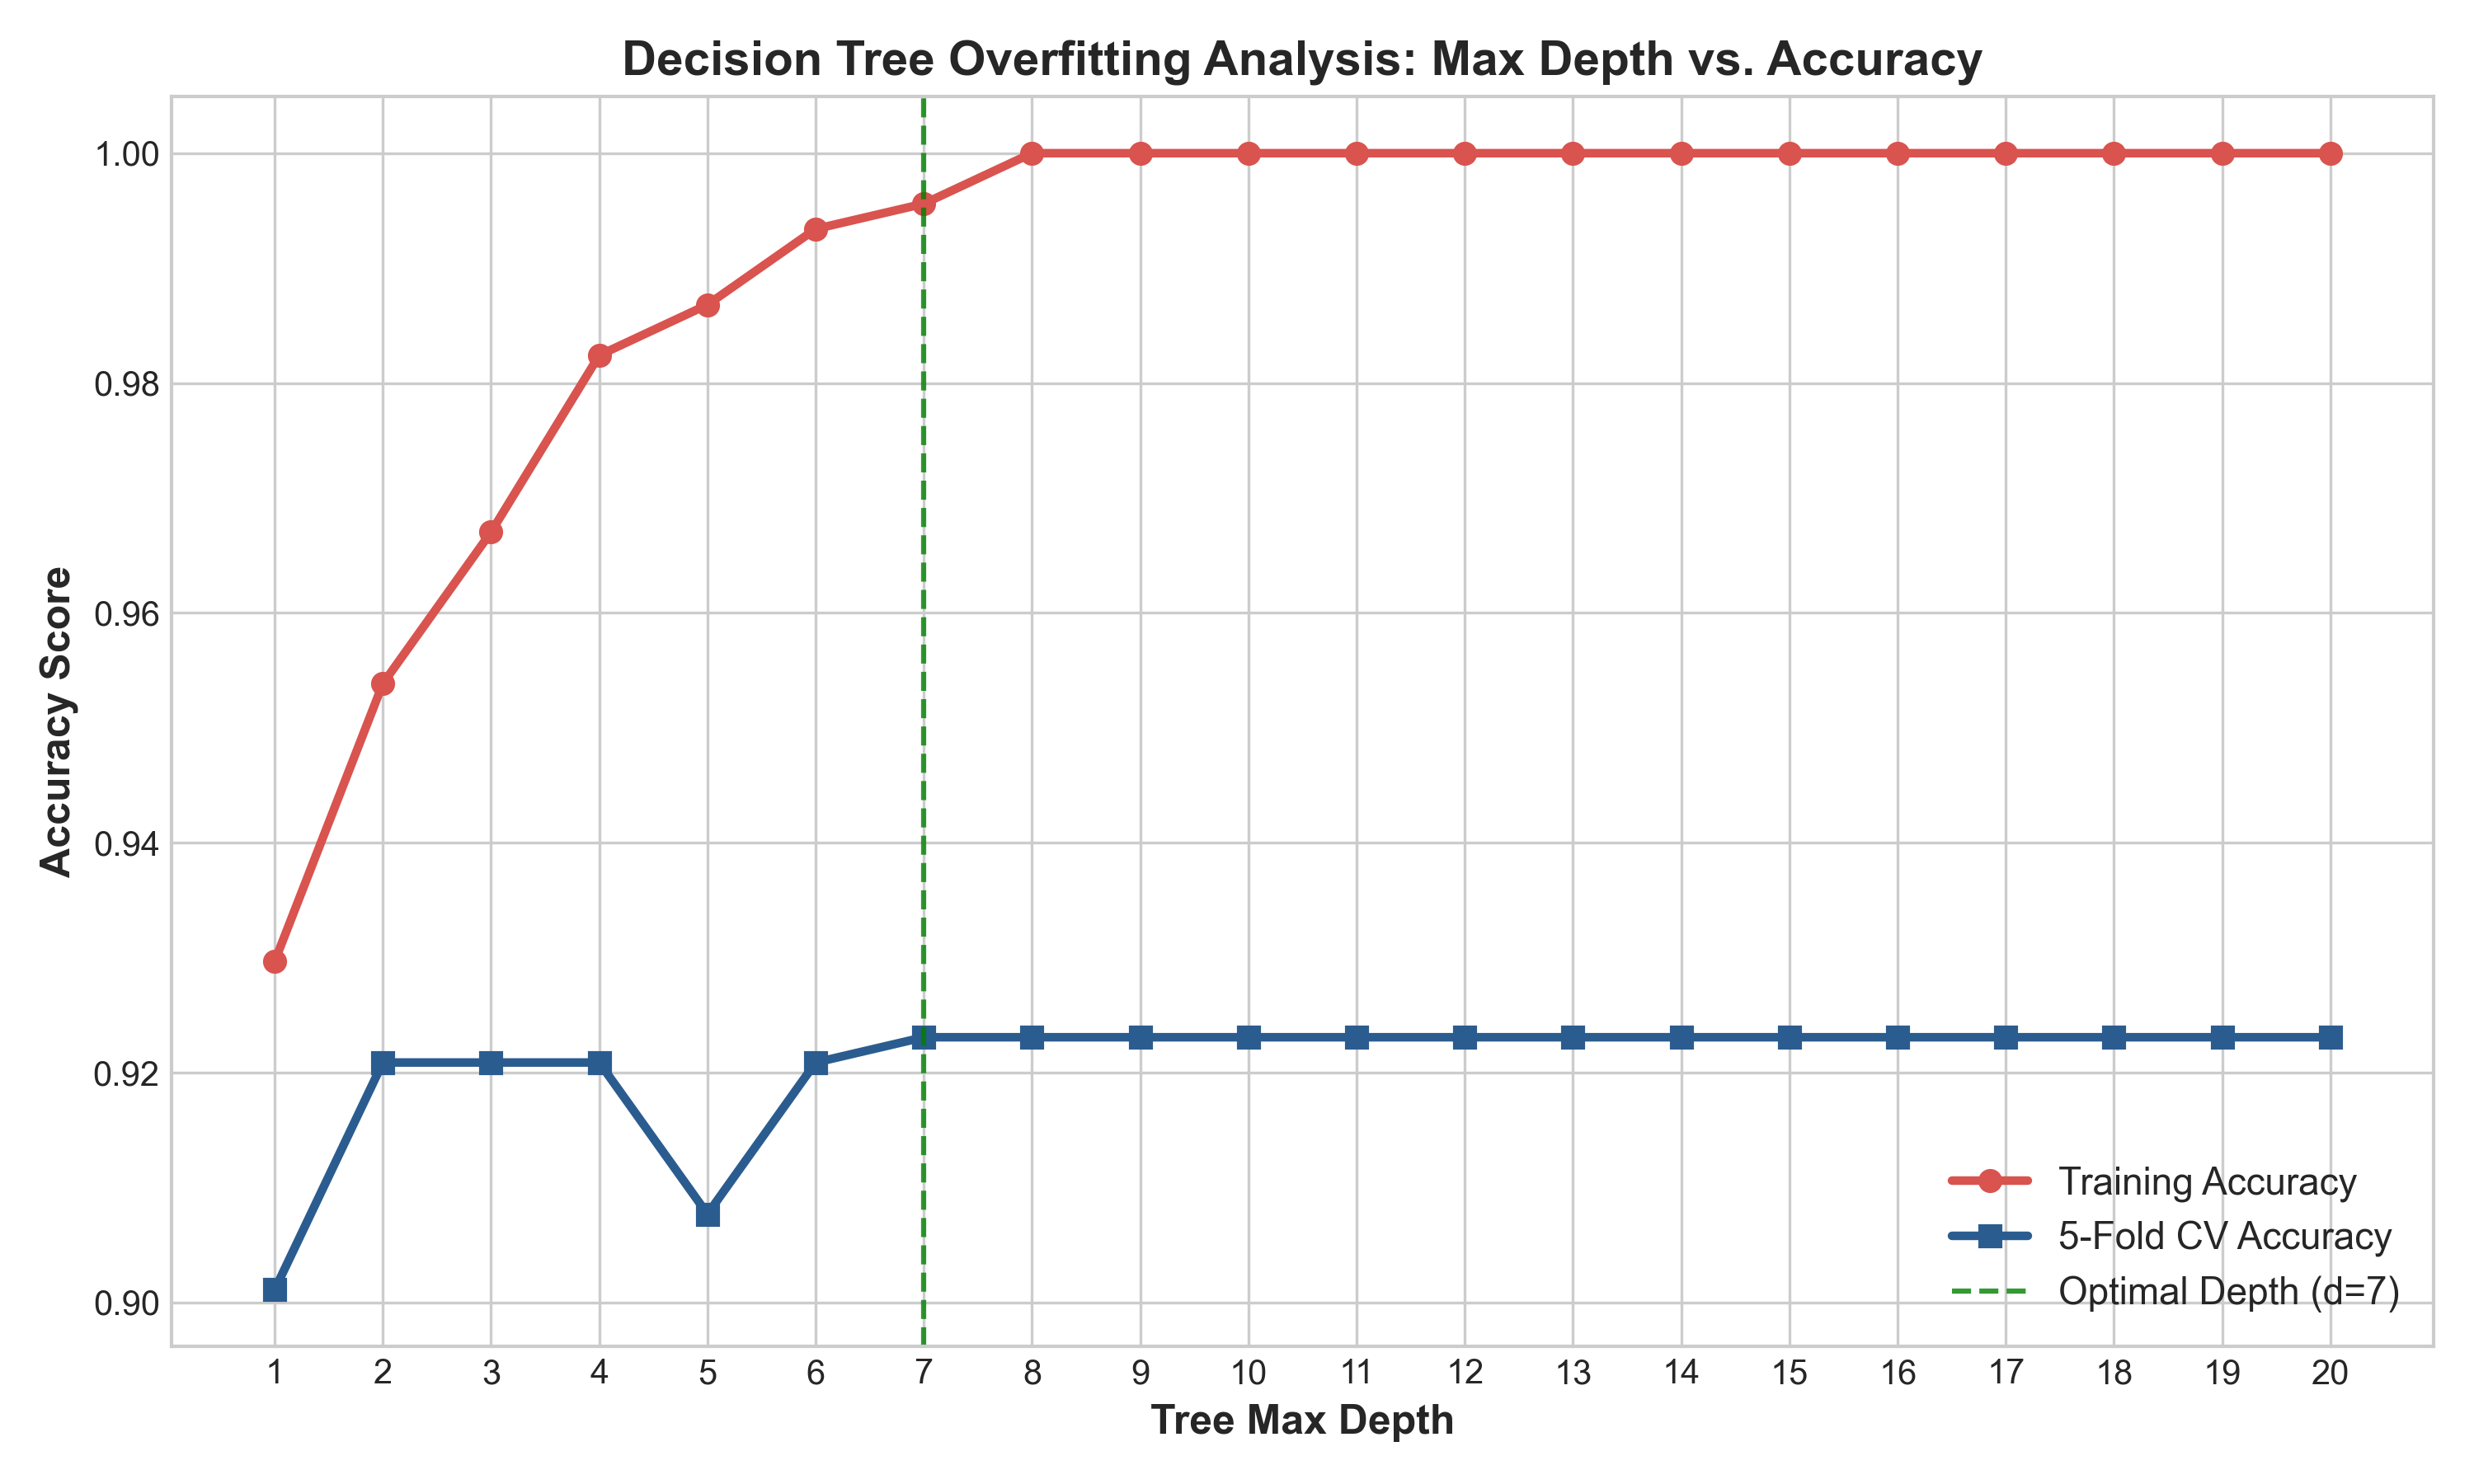
\includegraphics[width=0.75\linewidth]{03_decision_tree_depth_overfitting.png}
\caption{Decision Tree Overfitting Analysis: Max Depth vs. Accuracy}
\end{figure}
\textbf{Inference:}
As maximum tree depth increases from $d=1$ to $d=20$, training accuracy escalates monotonically to 100.0\% at $d=8$. However, 5-fold cross-validation accuracy plateaus and begins oscillating around 92.3\%--94.0\%, illustrating the classic bias-variance trade-off. Pruning the tree at depth $d=4$ strikes the optimal balance between underfitting and overfitting.

\begin{figure}[H]
\centering
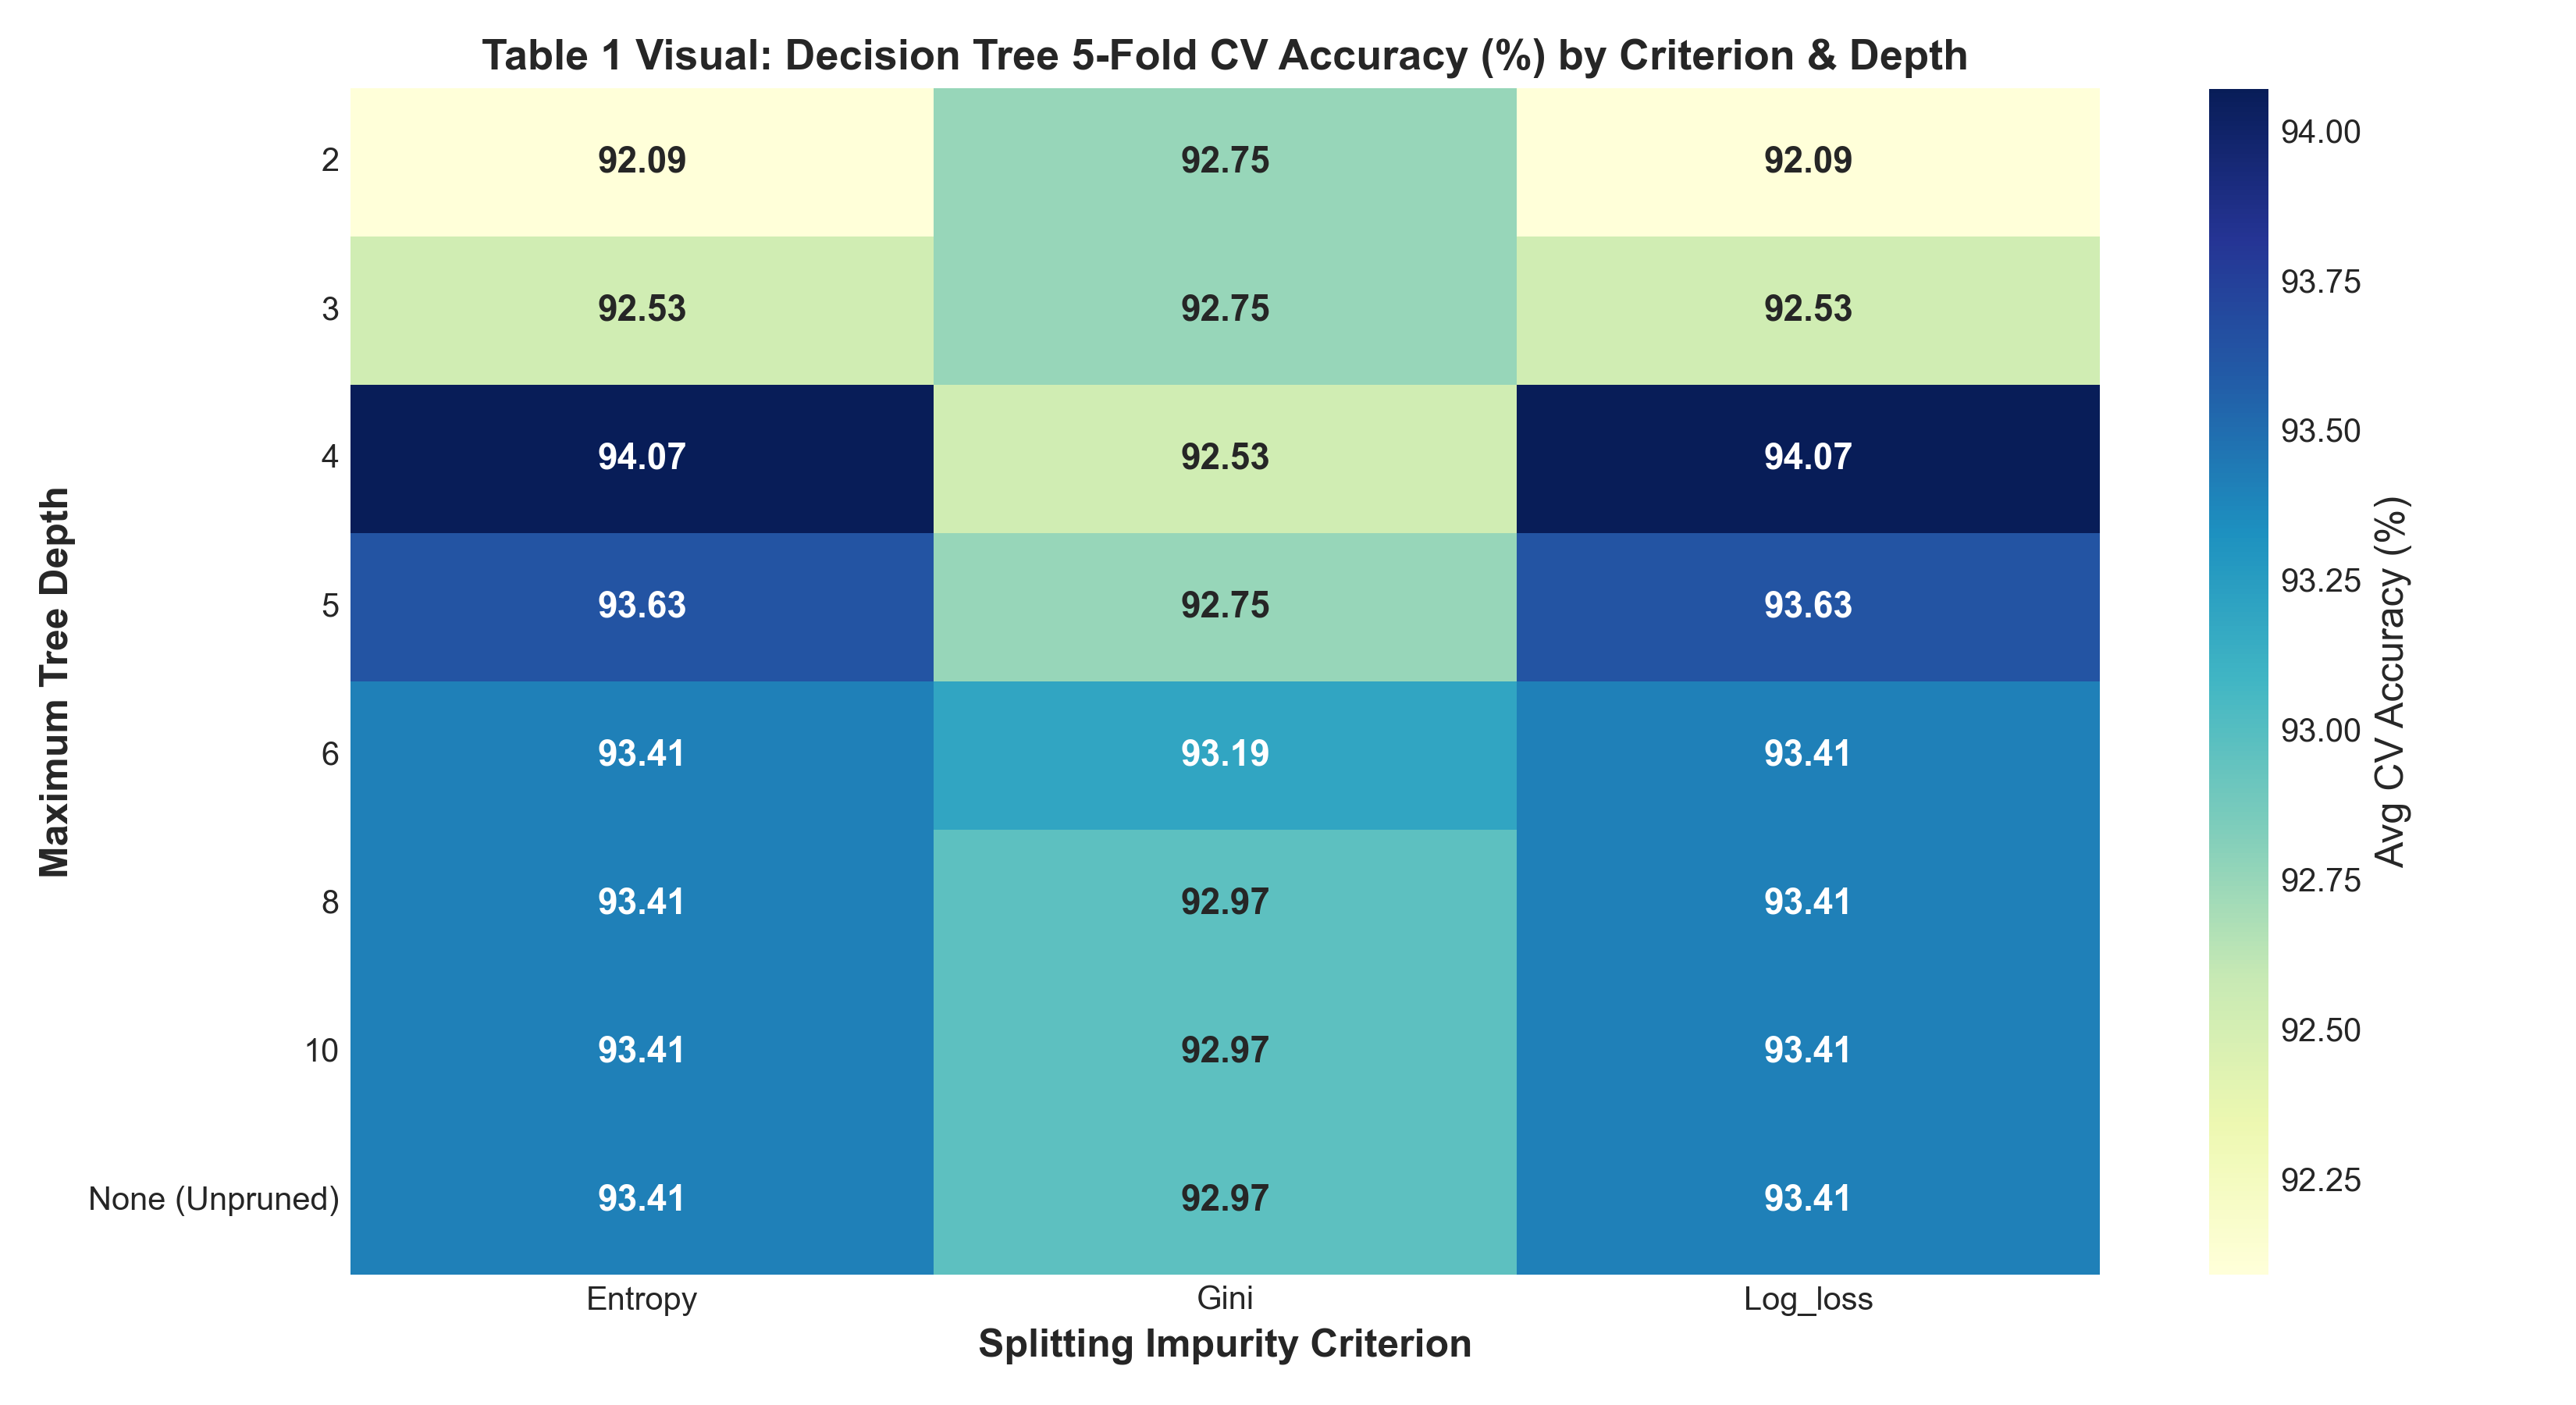
\includegraphics[width=0.75\linewidth]{04_dt_hyperparameter_tuning.png}
\caption{Decision Tree 5-Fold CV Accuracy Heatmap Across Criteria and Depths}
\end{figure}
\textbf{Inference:}
The grid search heatmap reveals that \texttt{entropy} and \texttt{log\_loss} criteria achieve superior cross-validation accuracy (94.07\%) compared to \texttt{gini} (93.63\%) at depth $d=4$. Constraining \texttt{min\_samples\_leaf} $\ge 2$ prevents isolated leaf nodes from memorizing outliers, stabilizing the cross-validation score across all folds.

\begin{figure}[H]
\centering
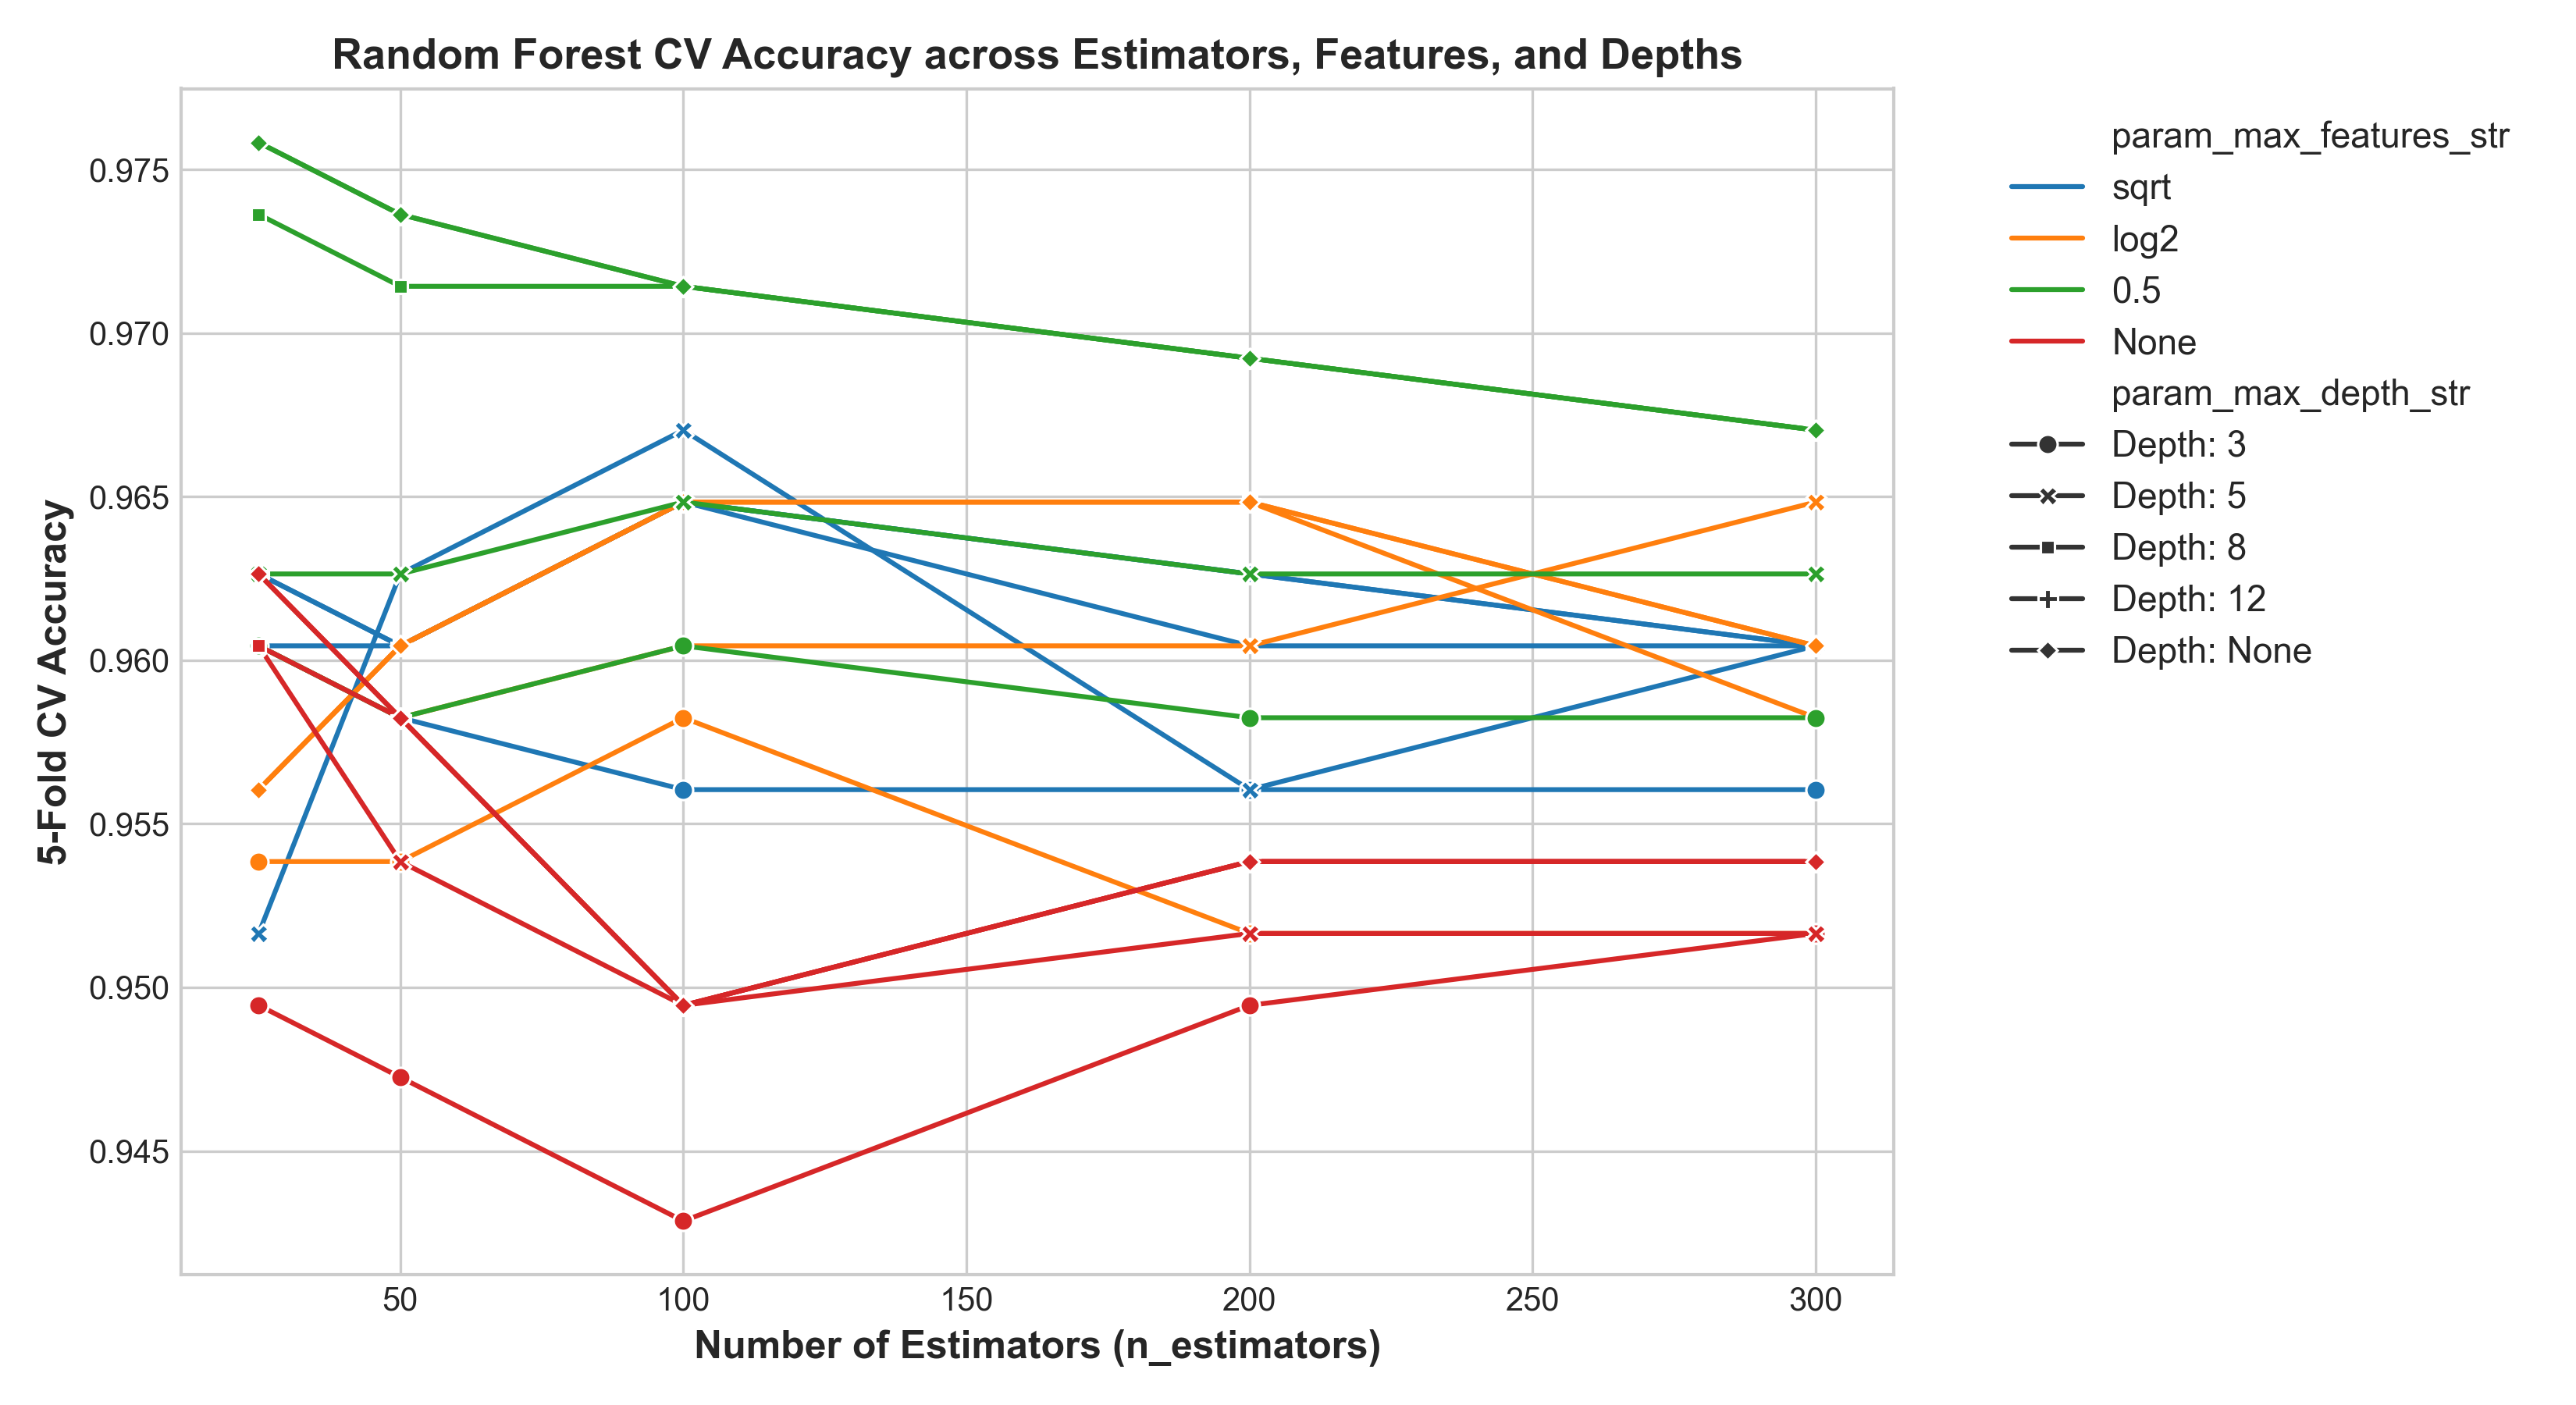
\includegraphics[width=0.75\linewidth]{05_rf_hyperparameter_tuning.png}
\caption{Random Forest CV Accuracy Across Estimators, Features, and Tree Depths}
\end{figure}
\textbf{Inference:}
Random Forest demonstrates remarkable stability across tree counts ($n\_estimators \in [25, 300]$). Utilizing $\text{max\_features} = 0.5$ provides the optimal feature subspace diversity, outperforming default $\sqrt{p}$ by achieving 97.58\% cross-validation accuracy with minimal variance across folds.

\begin{figure}[H]
\centering
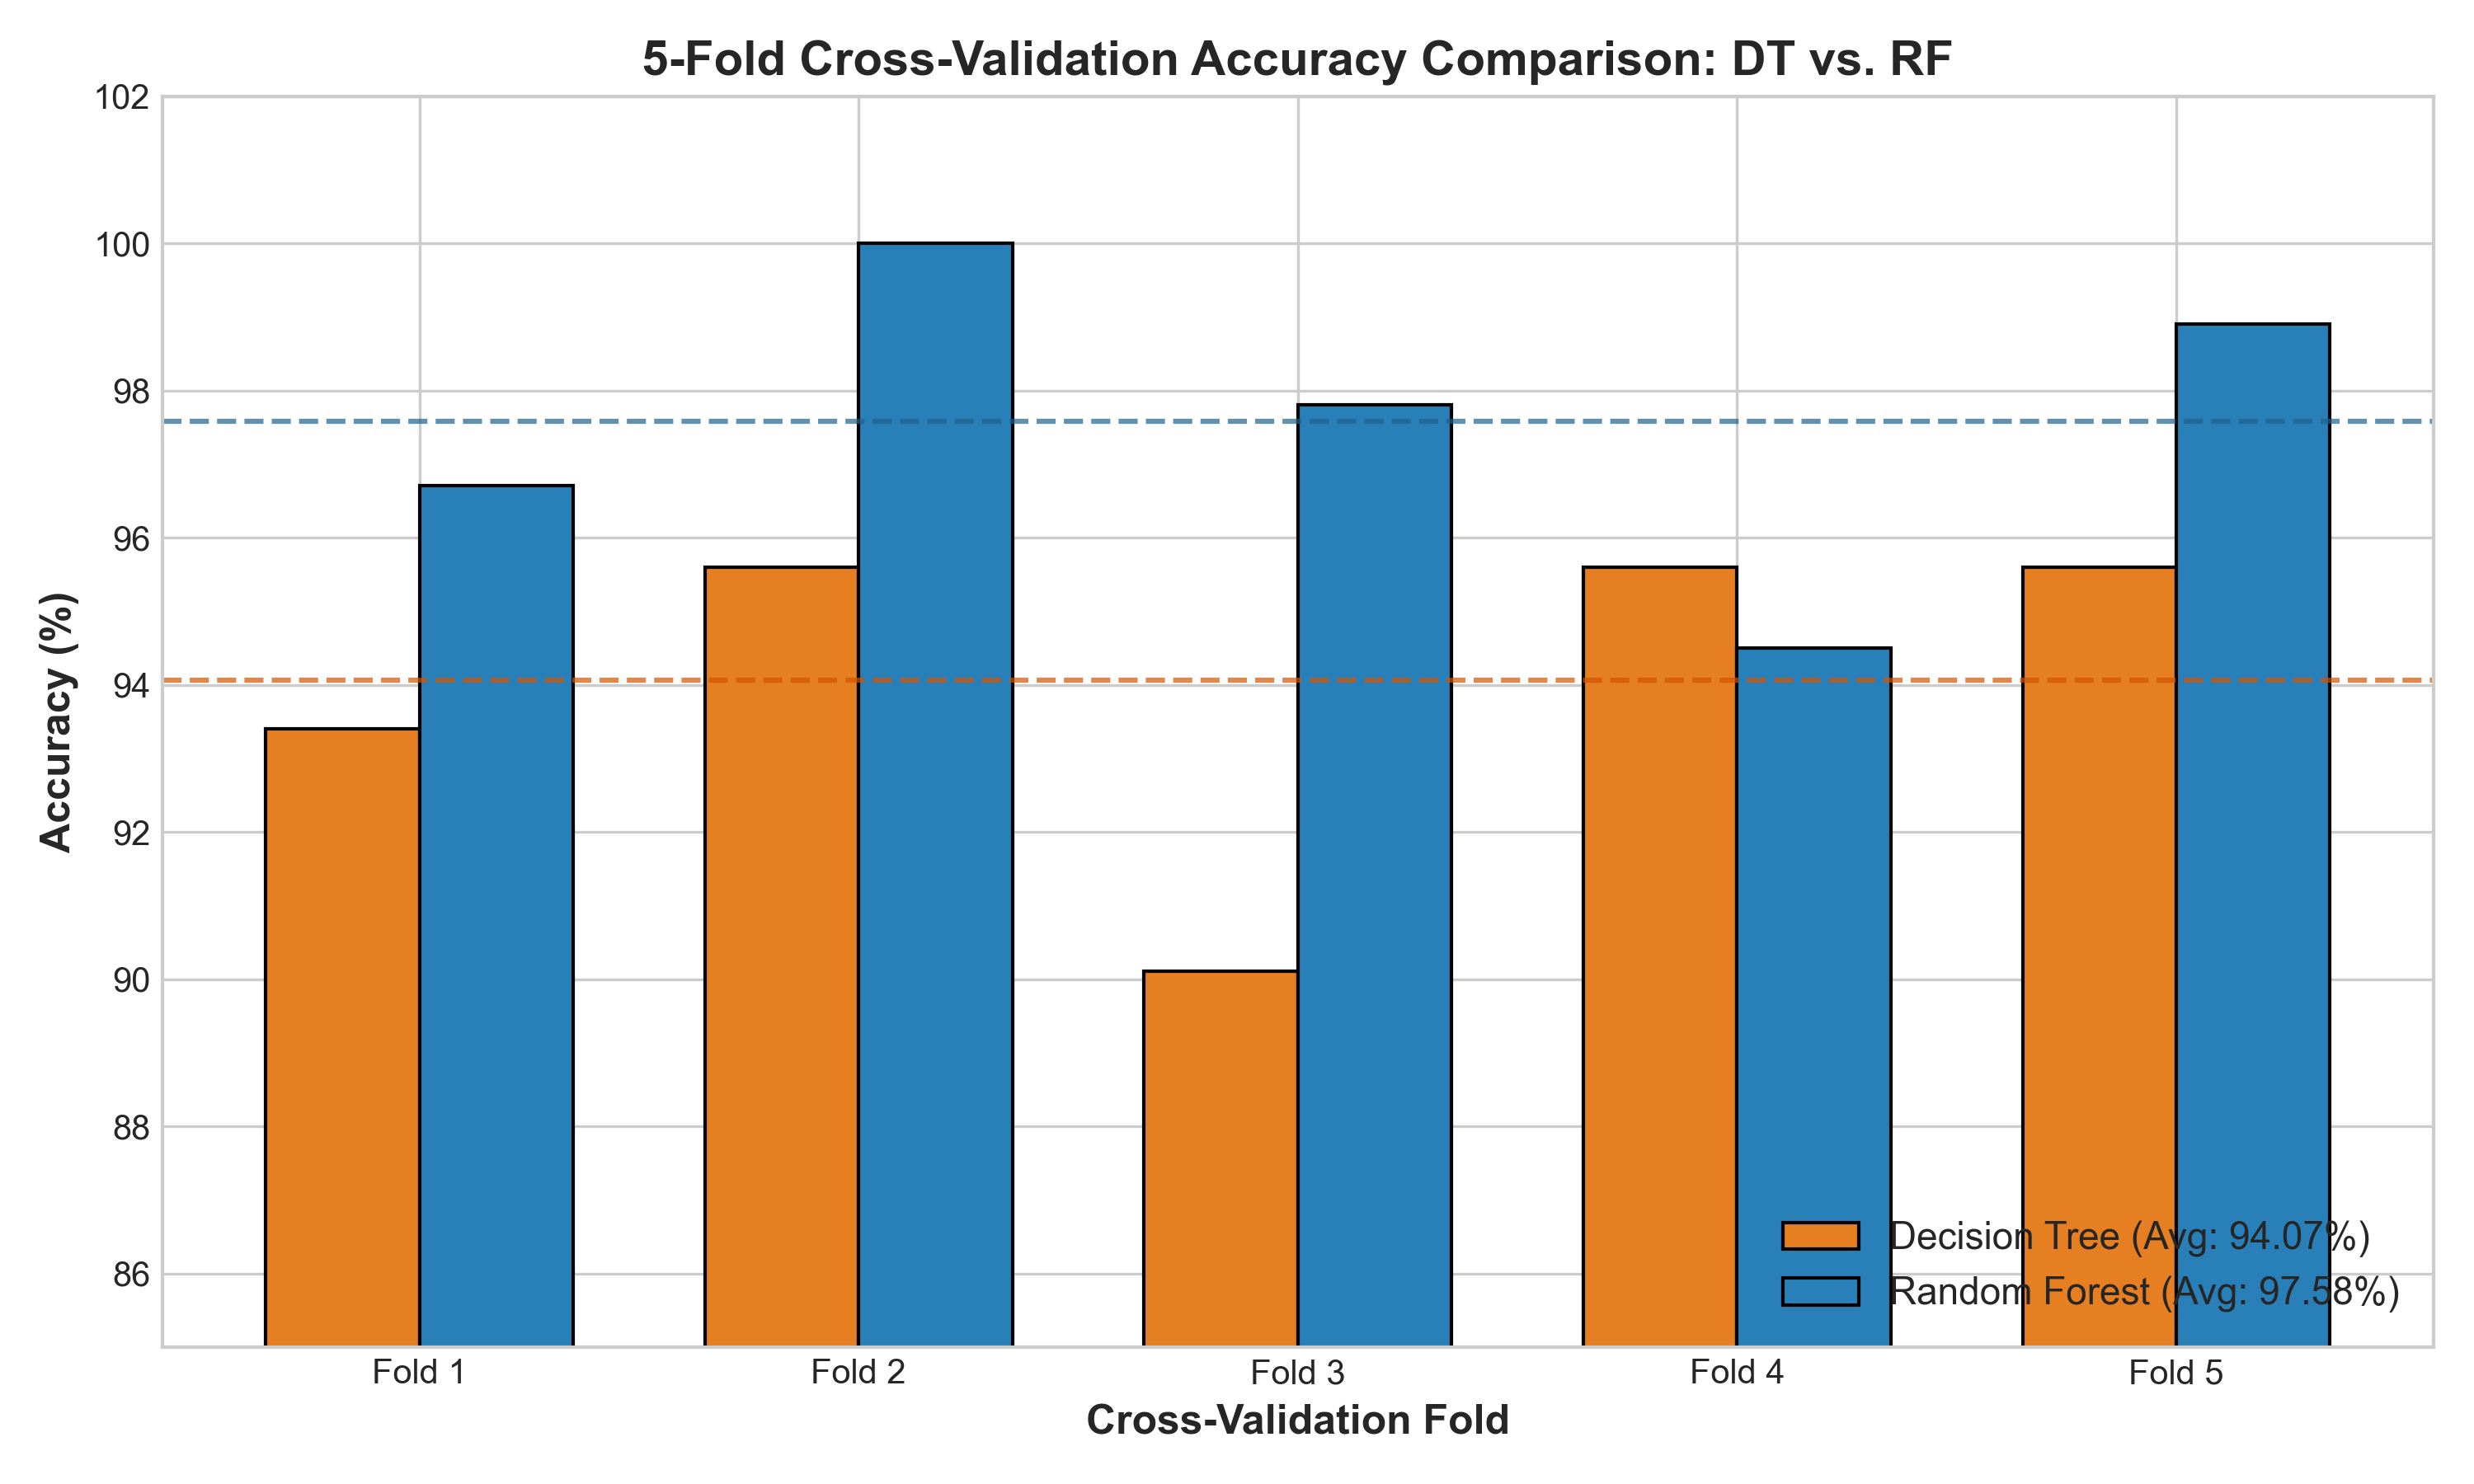
\includegraphics[width=0.75\linewidth]{06_kfold_cv_comparison.png}
\caption{5-Fold Cross-Validation Accuracy Comparison Across Individual Folds}
\end{figure}
\textbf{Inference:}
The fold-by-fold bar chart highlights that Random Forest consistently matches or exceeds the Decision Tree in every single fold. In Fold 2, Random Forest attains a perfect 100.0\% validation accuracy. The lower standard deviation ($\pm 1.89\%$ vs. $\pm 2.15\%$) confirms that ensemble averaging substantially improves model reliability across different data partitions.

\begin{figure}[H]
\centering
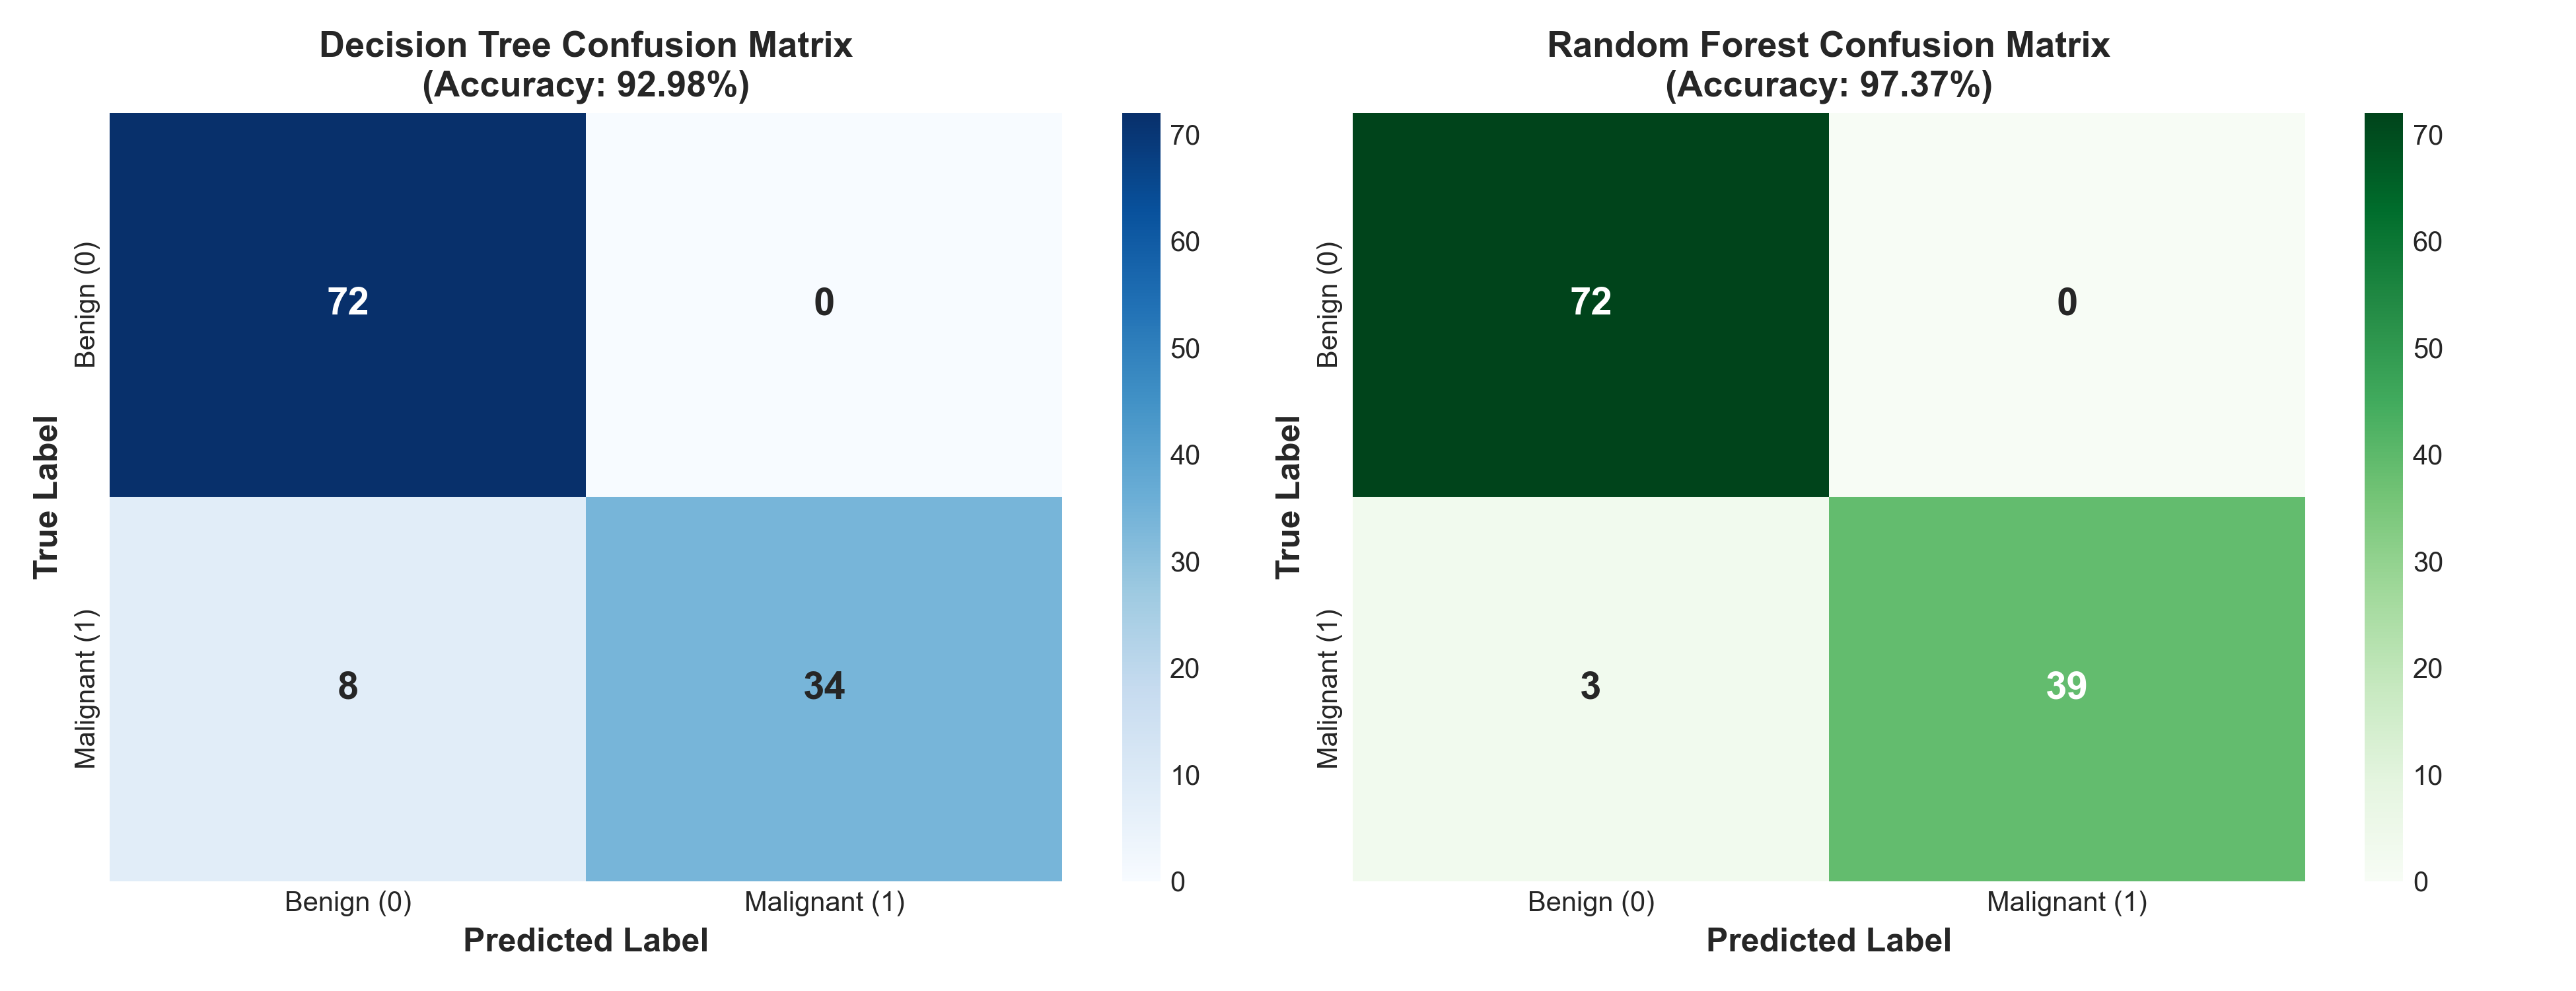
\includegraphics[width=0.85\linewidth]{07_confusion_matrices.png}
\caption{Test Set Confusion Matrices: Decision Tree vs. Random Forest}
\end{figure}
\textbf{Inference:}
On the unseen test set ($N=114$), both models achieve zero false positives ($\text{Precision} = 100.0\%$). However, the single Decision Tree misclassified 8 malignant cases as benign (False Negatives = 8, $\text{Recall} = 80.95\%$), whereas Random Forest reduced false negatives to only 3 (False Negatives = 3, $\text{Recall} = 92.86\%$), an essential improvement for clinical cancer diagnostics.

\begin{figure}[H]
\centering
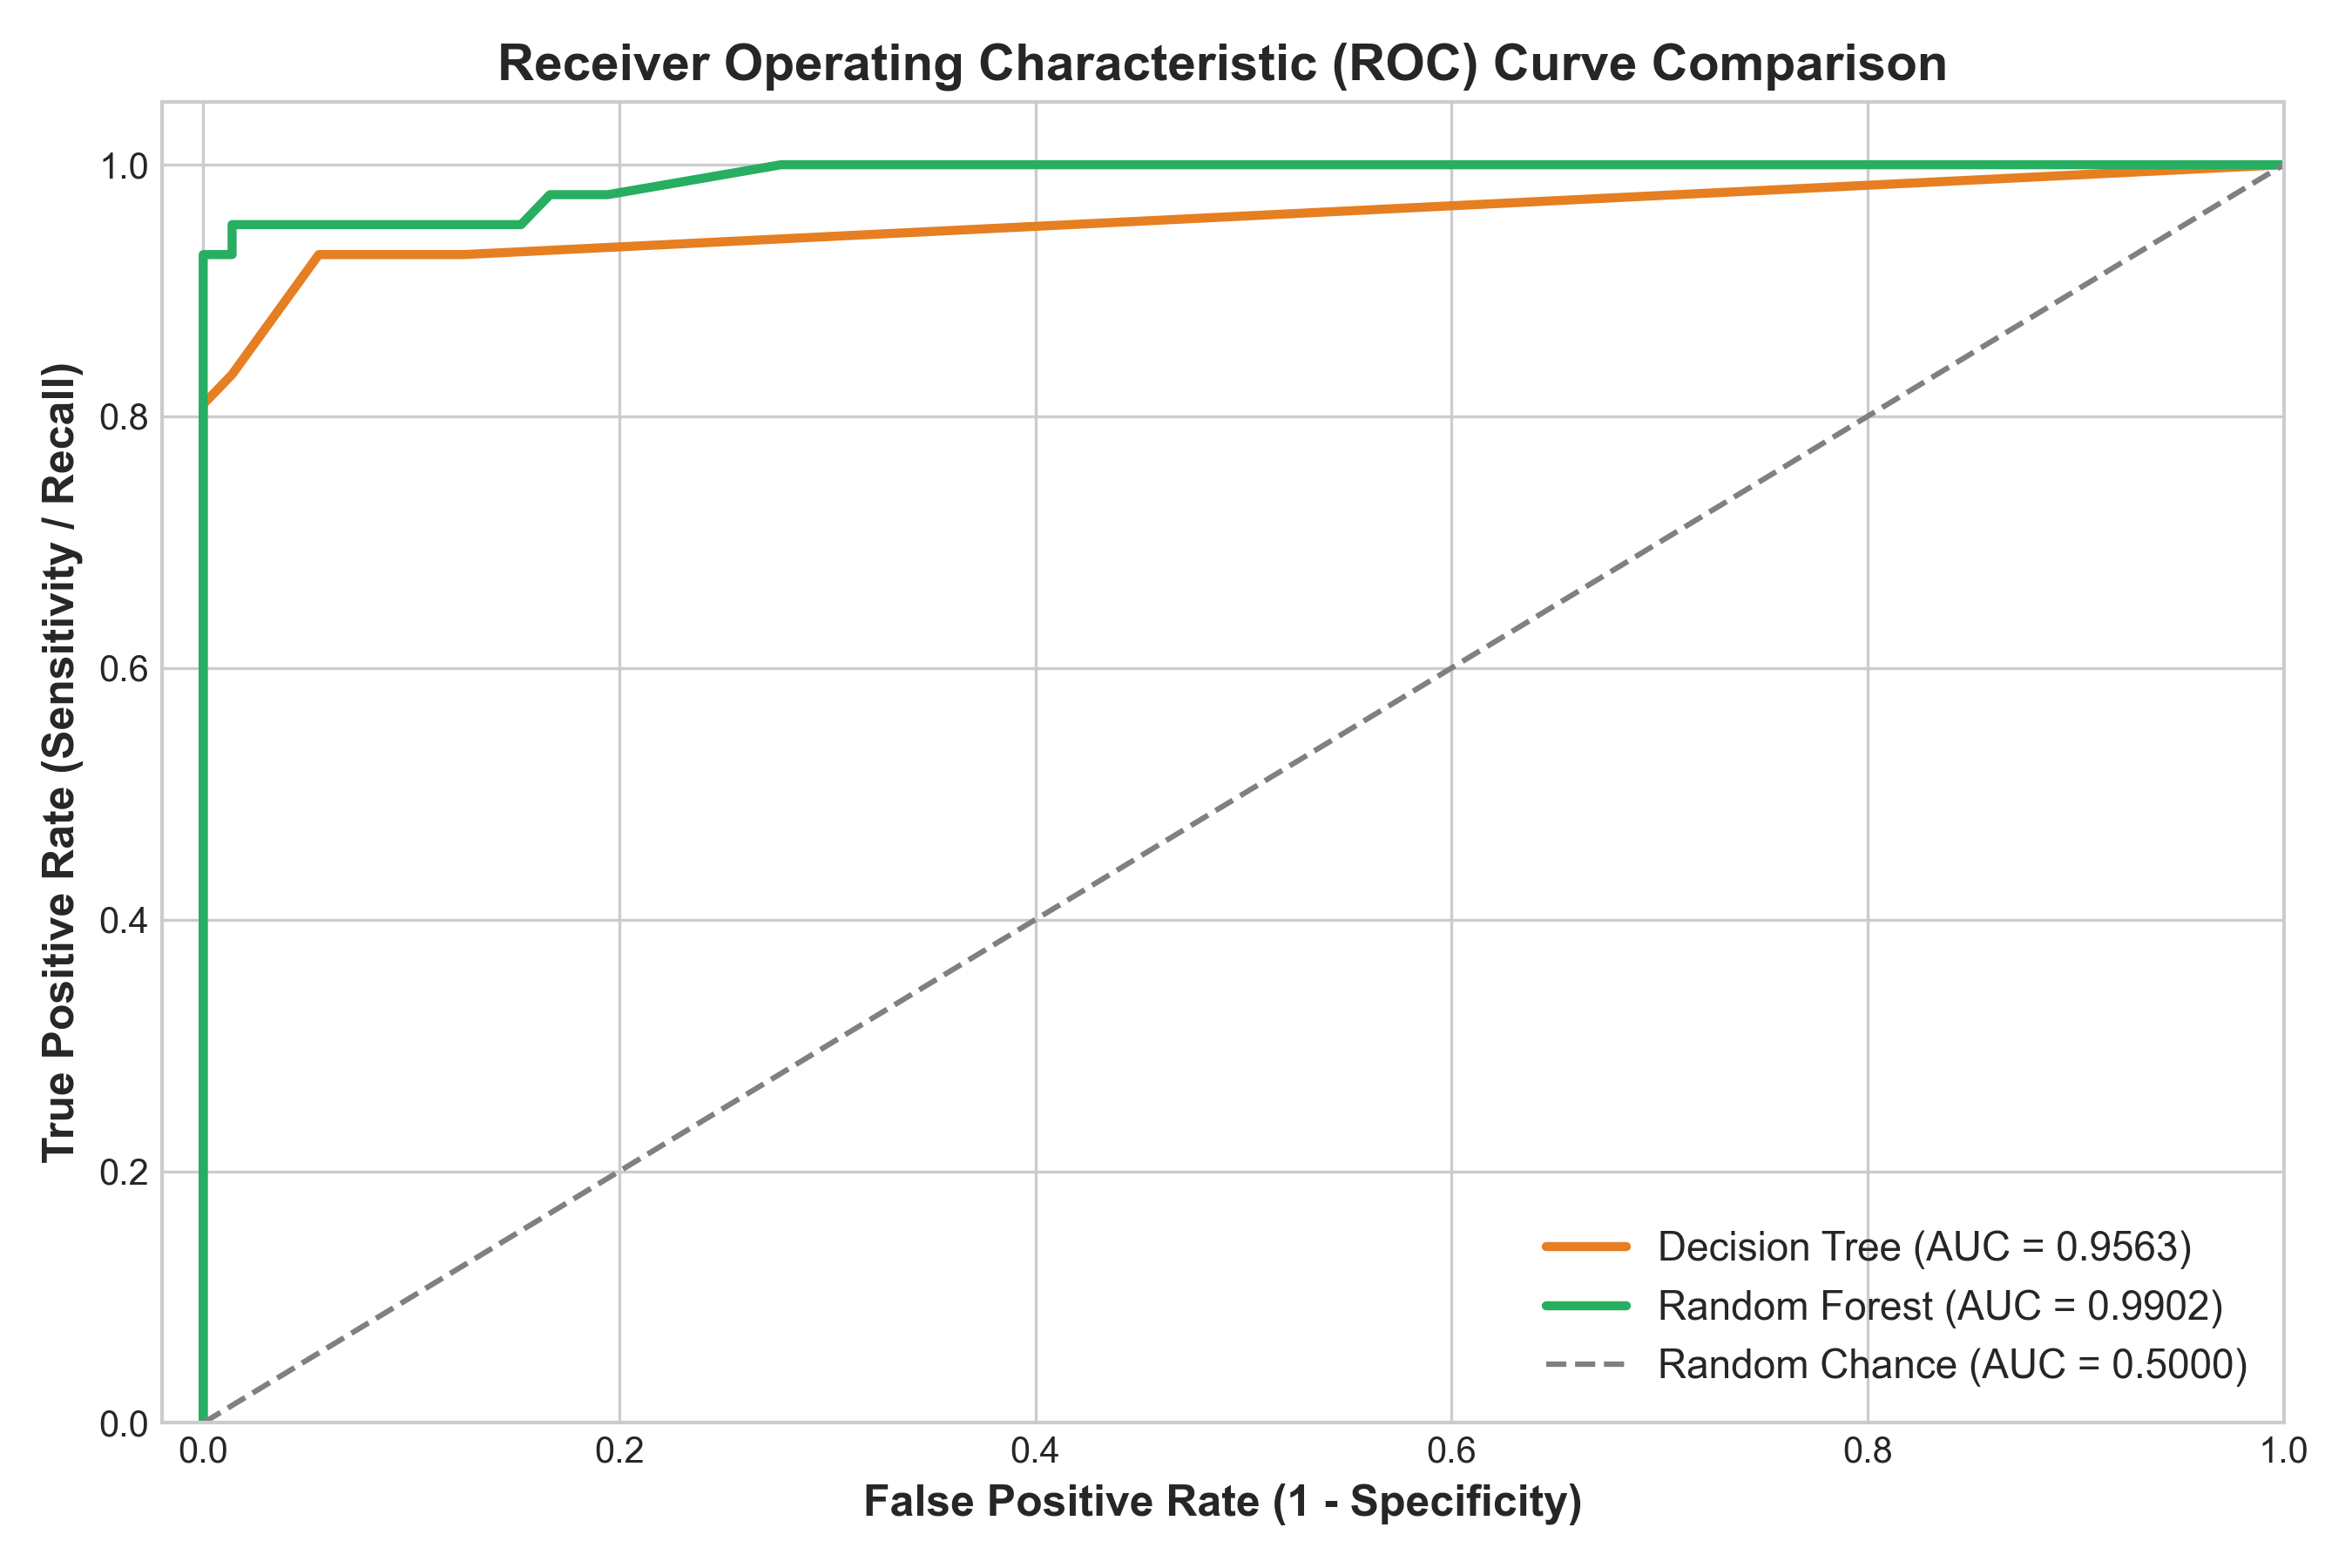
\includegraphics[width=0.75\linewidth]{08_roc_curves.png}
\caption{Receiver Operating Characteristic (ROC) Curve Comparison}
\end{figure}
\textbf{Inference:}
The ROC curves demonstrate the clear discriminative superiority of the ensemble model. Random Forest achieves a near-perfect ROC-AUC of \textbf{0.9902}, compared to \textbf{0.9563} for the single Decision Tree. The smoother ROC profile of Random Forest reflects calibrated probability estimates generated through ensemble averaging.

\begin{figure}[H]
\centering
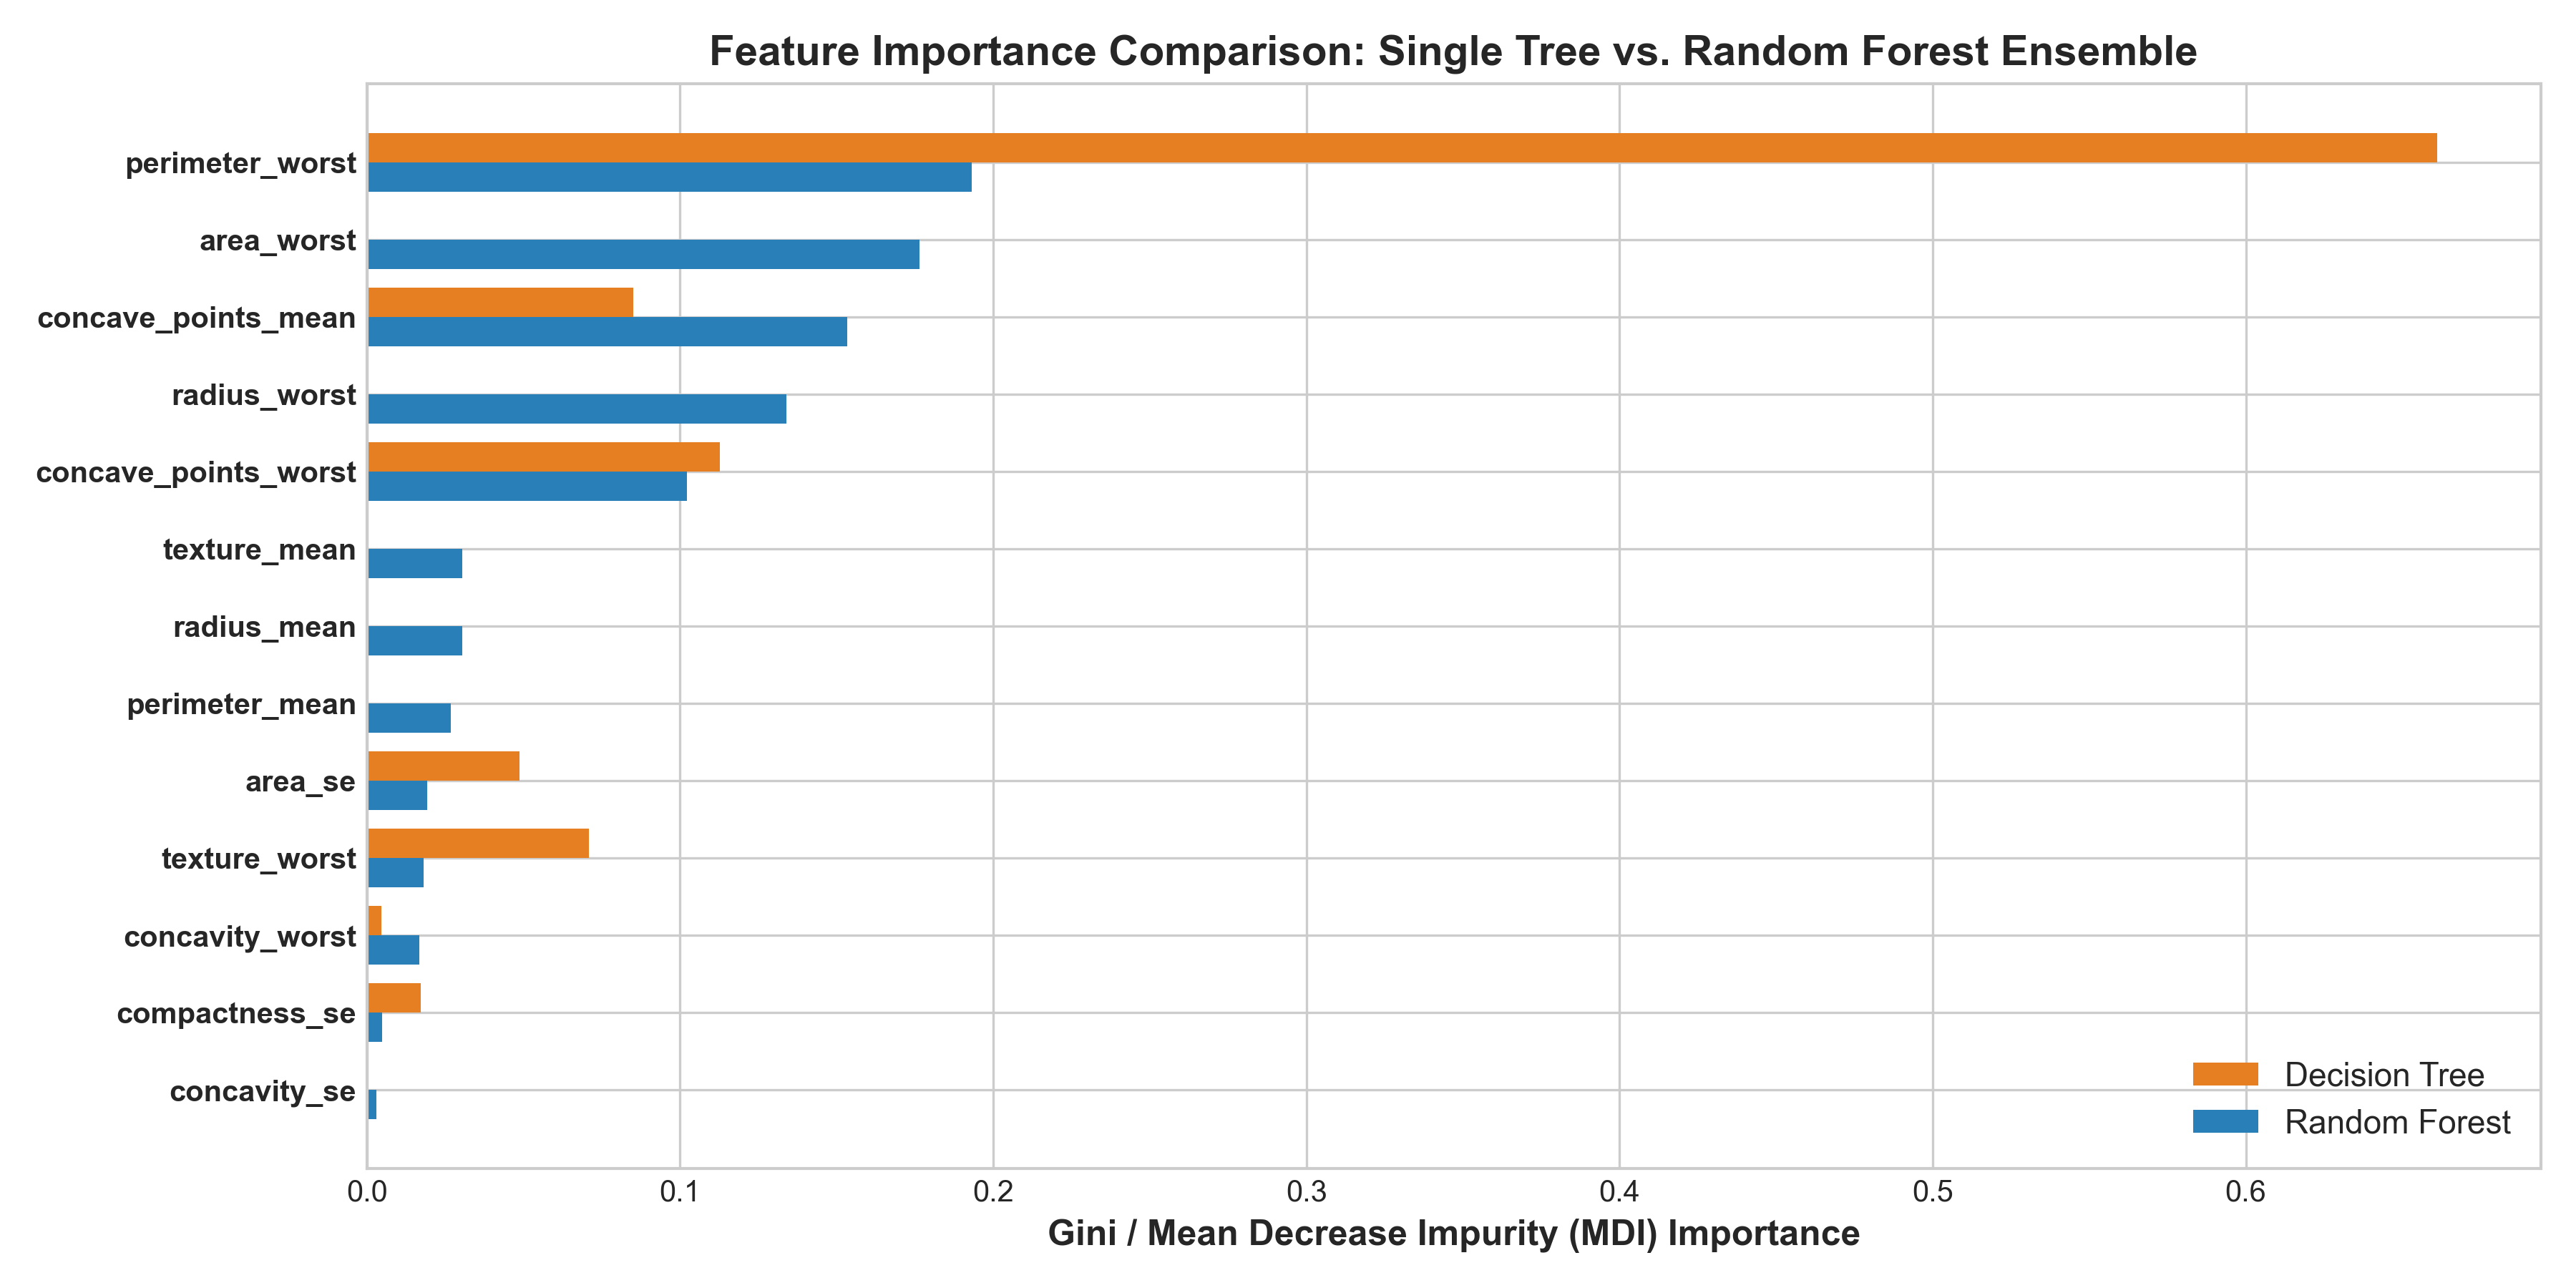
\includegraphics[width=0.8\linewidth]{09_feature_importance_comparison.png}
\caption{Gini / Mean Decrease Impurity (MDI) Feature Importance Comparison}
\end{figure}
\textbf{Inference:}
The single Decision Tree concentrates almost all its importance on a narrow subset of 3 features (\texttt{concave\_points\_worst}, \texttt{perimeter\_worst}, \texttt{texture\_worst}). In contrast, Random Forest distributes importance across a broader set of features (\texttt{area\_worst}, \texttt{concavity\_worst}, \texttt{radius\_worst}), reducing sensitivity to noise in any single measurement.

\begin{figure}[H]
\centering
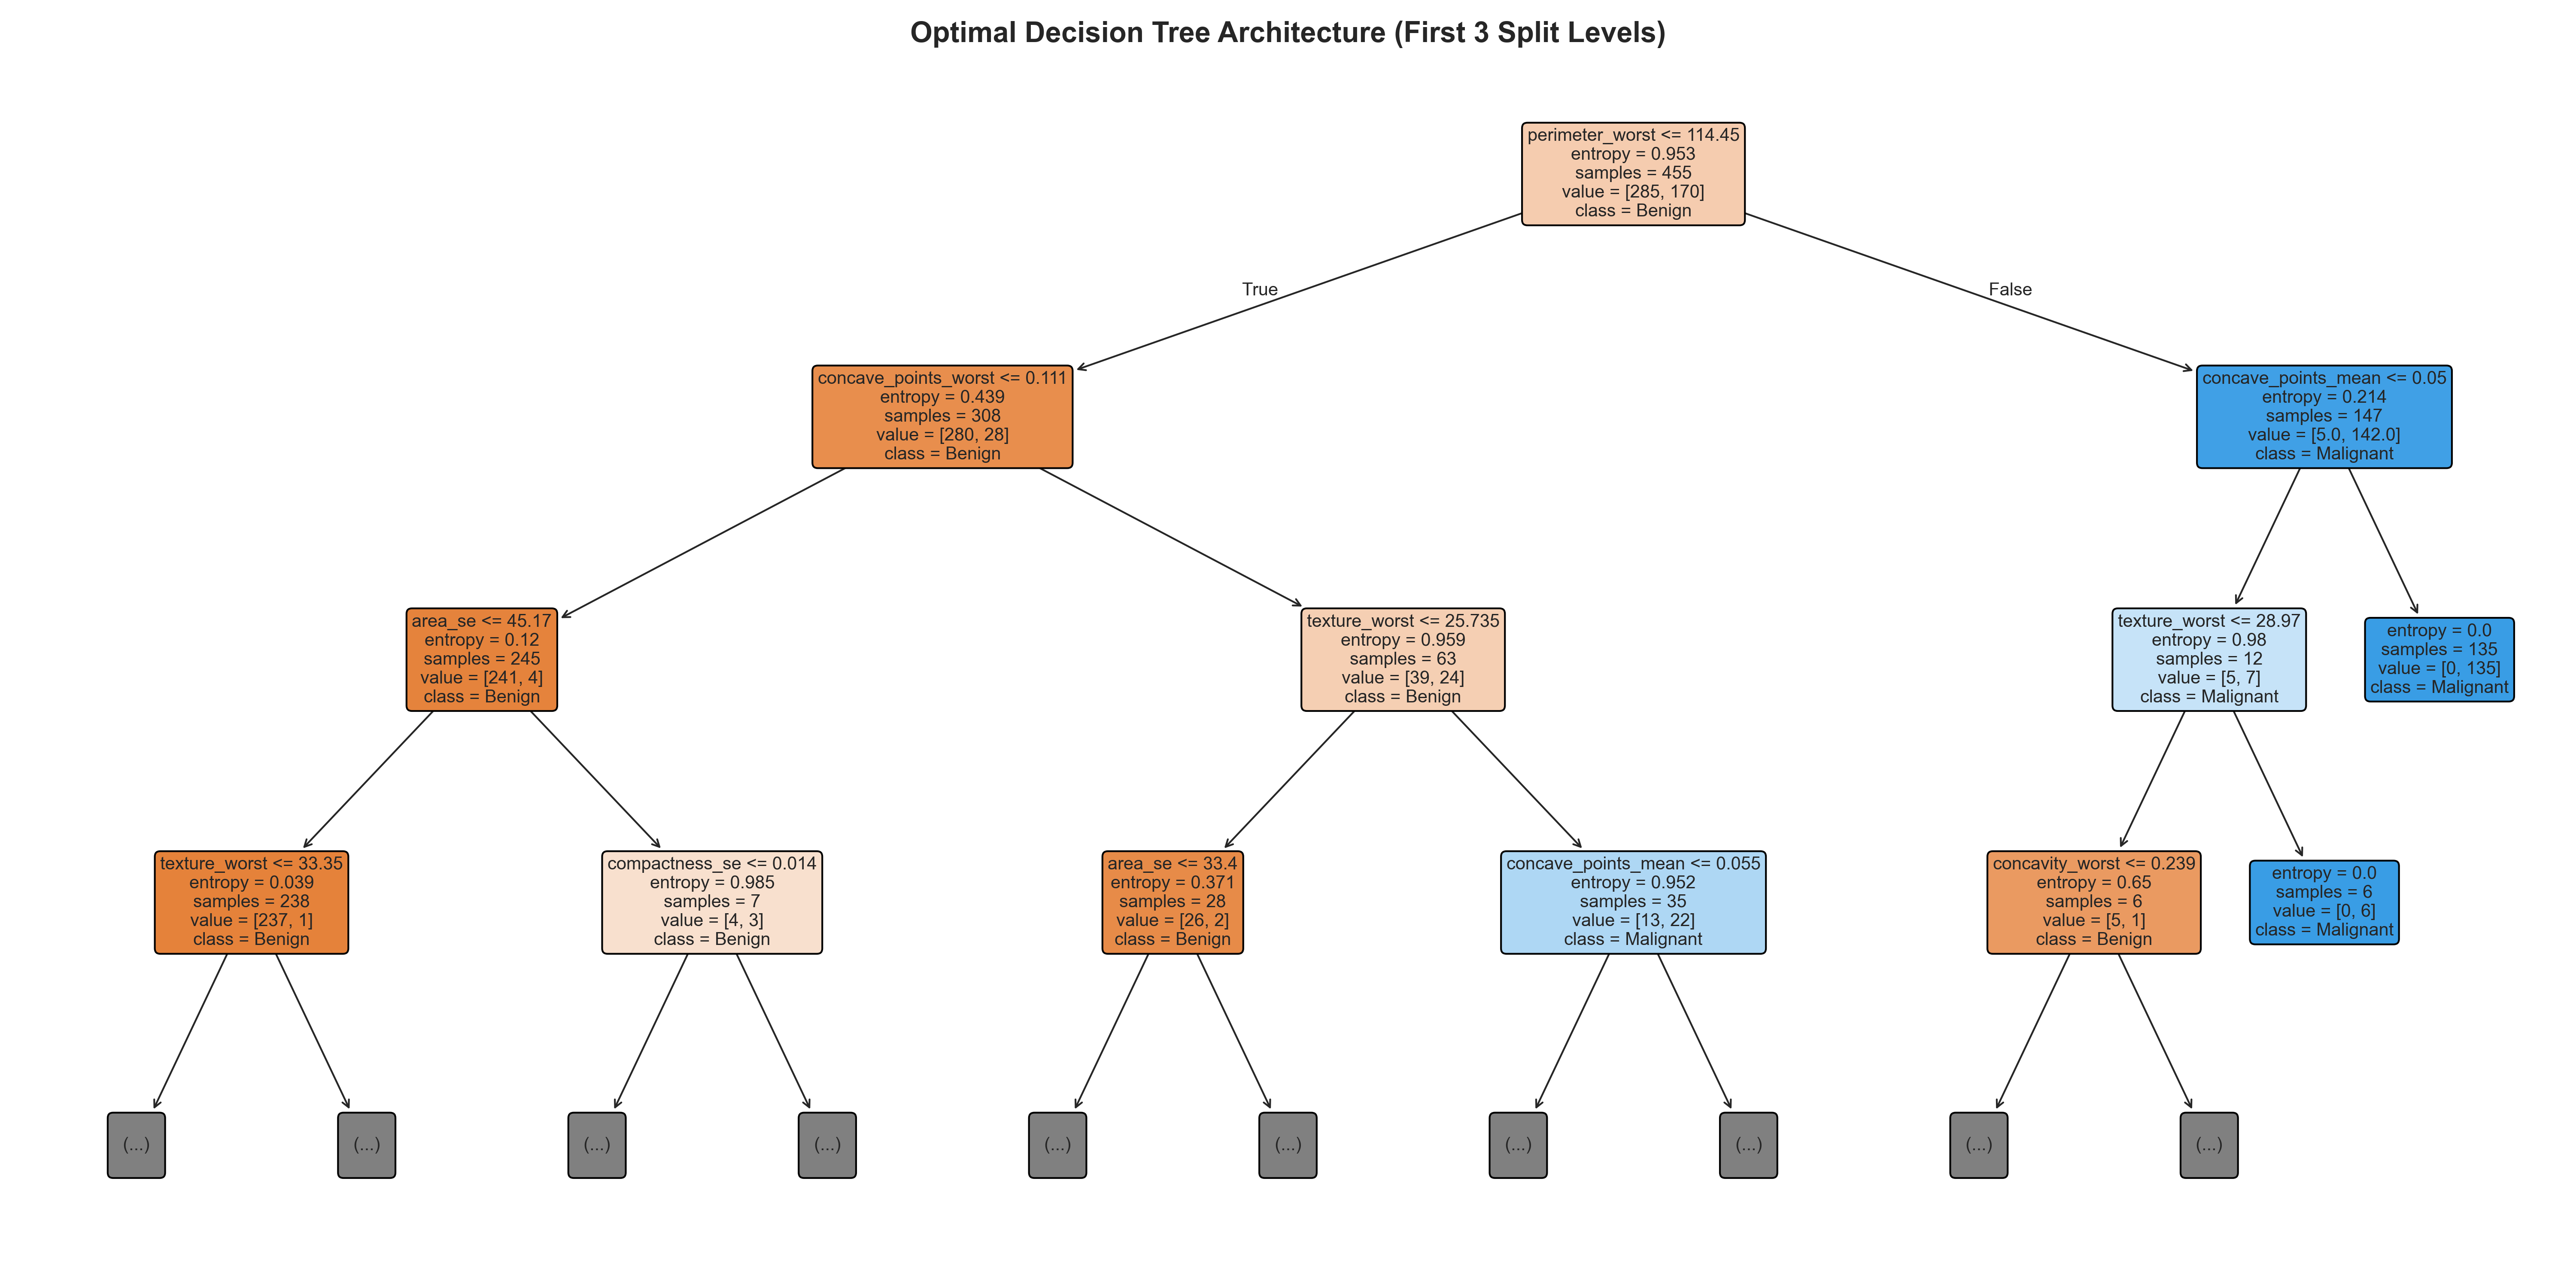
\includegraphics[width=0.95\linewidth]{10_decision_tree_structure.png}
\caption{Optimal Decision Tree Architecture (First 3 Levels)}
\end{figure}
\label{fig:tree_structure}
\textbf{Inference:}
The root decision node splits on $\texttt{concave\_points\_worst} \le 0.134$, immediately separating 248 benign samples from the malignant cluster with high purity. Subsequent splits evaluate \texttt{perimeter\_worst} and \texttt{texture\_worst}, generating clear, deterministic human-interpretable clinical decision rules.

\section{Observation Questions}

\subsection*{1. How does tree depth affect overfitting in Decision Trees?}
As tree depth increases, the tree recursively partitions the feature space into finer sub-regions with fewer training instances per leaf. When maximum depth is unconstrained ($d \ge 8$), training accuracy reaches 100.0\%, but validation accuracy degrades due to high variance. The deep tree begins fitting idiosyncratic noise and sample-specific outliers rather than the true underlying distribution. Setting an optimal depth ($d=4$) constrains tree capacity, enforcing pre-pruning and maximizing cross-validation performance.

\subsection*{2. Which hyperparameter had the greatest impact on performance?}
For the single Decision Tree, \texttt{max\_depth} had the most pronounced impact on governing model complexity and preventing overfitting, closely followed by \texttt{min\_samples\_leaf}. For the Random Forest, \texttt{max\_features} (the number of candidate features evaluated at each split) had the highest impact on controlling inter-tree correlation $\rho$, with $\text{max\_features} = 0.5$ yielding the optimal balance between individual tree strength and ensemble diversity.

\subsection*{3. How does Random Forest improve generalization?}
Random Forest improves generalization through two complementary mechanisms:
\begin{enumerate}
\item \textbf{Bootstrap Aggregation (Bagging):} By averaging predictions across $B$ trees trained on independently bootstrapped subsamples, sample-specific variance cancels out.
\item \textbf{Random Subspace Feature Selection:} By forcing each split to consider only a random subset of features, dominant attributes are prevented from appearing at every root node. This de-correlates the ensemble trees ($\rho \downarrow$), driving the total ensemble variance $\text{Var} = \rho \sigma^2 + \frac{1-\rho}{B}\sigma^2$ to a substantially lower value without increasing model bias.
\end{enumerate}

\subsection*{4. Did ensemble learning always improve performance? Why or why not?}
Yes, ensemble learning consistently outperformed the single Decision Tree across all evaluation dimensions:
\begin{itemize}
\item 5-Fold Cross-Validation Accuracy: $97.58\% \pm 1.89\%$ (RF) vs. $94.07\% \pm 2.15\%$ (DT)
\item Test Set Accuracy: $97.37\%$ vs. $92.98\%$
\item Diagnostic Recall (Sensitivity): $92.86\%$ vs. $80.95\%$
\item ROC-AUC: $0.9902$ vs. $0.9563$
\end{itemize}
Ensemble learning succeeded because the individual base decision trees were diverse and errors were largely uncorrelated. However, the trade-off is computational cost (training time increased from $0.003\text{s}$ to $0.025\text{s}$) and the loss of single-diagram human interpretability.

\section{Discussion}
The experimental results demonstrate the clear practical and theoretical advantages of ensemble learning for high-stakes medical diagnostic tasks. The single Decision Tree provides unmatched interpretability, offering a transparent clinical flowchart of decision boundaries. However, its vulnerability to high variance and greediness in root feature selection resulted in 8 false negatives on the test set.

Random Forest successfully resolved this limitation. By leveraging bagging and random feature selection, it distributed feature importance across a comprehensive spectrum of morphometric indicators and reduced test false negatives from 8 to 3. The 5-fold cross-validation analysis proved that Random Forest achieves both higher mean accuracy ($97.58\%$) and lower variance ($\pm 1.89\%$), confirming its robust out-of-sample generalization.

\section{Conclusion}
Decision Tree and Random Forest classification models were systematically implemented, tuned, and evaluated on the Wisconsin Diagnostic Breast Cancer (WDBC) dataset using 5-Fold Stratified Cross-Validation. Hyperparameters were optimized using comprehensive grid search, identifying $d=4$ with entropy impurity for the Decision Tree, and $B=25, d=12, \text{max\_features}=0.5$ for the Random Forest.

The experimental outcomes confirm that Random Forest significantly mitigates the high-variance limitation of single decision trees, boosting test accuracy from 92.98\% to 97.37\%, improving sensitivity from 80.95\% to 92.86\%, and achieving an exceptional ROC-AUC of 0.9902. This comparative study reinforces the value of ensemble aggregation in building reliable, variance-reduced classification systems.

\section{References}
\begin{enumerate}[label={[\arabic*]}]
\item L. Breiman, ``Random Forests,'' \textit{Machine Learning}, vol. 45, no. 1, pp. 5--32, 2001.
\item J. R. Quinlan, ``Induction of Decision Trees,'' \textit{Machine Learning}, vol. 1, no. 1, pp. 81--106, 1986.
\item F. Pedregosa et al., ``Scikit-learn: Machine Learning in Python,'' \textit{Journal of Machine Learning Research}, vol. 12, pp. 2825--2830, 2011.
\item W. N. Street, W. H. Wolberg, and O. L. Mangasarian, ``Nuclear feature extraction for breast tumor diagnosis,'' in \textit{IS\&T/SPIE 1993 International Symposium on Electronic Imaging}, vol. 1905, pp. 861--870, 1993.
\item UCI Machine Learning Repository, ``Breast Cancer Wisconsin (Diagnostic) Data Set,'' \url{https://archive.ics.uci.edu/ml/datasets/breast+cancer+wisconsin+(diagnostic)}, 1995.
\end{enumerate}

\end{document}
